\chapter{函数与极限}
\markboth{函数与极限}{函数与极限}

\begin{remark}[本章定位]\label{rem:function_chapter_positioning}
数学的研究对象是量与形，而函数是描述量与量之间关系的核心工具。本章从函数的基本定义出发，逐步展开极限、连续性、导数、微分与积分的分析理论，为后续章节的严格论证提供分析基础。

本章的核心工作之一，是将“标量与矢量”章中建立的\textbf{相似度与趋势谱系}从三角函数层面扩充到微积分层面。在向量层面，相似度通过两向量的辐角差/和来计算。在函数层面，我们引入\textbf{极限角}的概念——函数在一点处的导数即该点切线方向的正切值（$f'(a) = \tan\theta_a$），从而将辐角差/和的计算转化为极限角差/和的计算。这一扩充使得相似度和趋势不再依赖于具体的三角函数形式，而是通过\textbf{微分和积分}直接计算，适用范围从离散向量推广到连续函数。

\textbf{本章七主题导引}：平移——导数（方向信息）与极限角 $\theta_f(a)=\arctan f'(a)$；缩放——积分（趋势信息）与对数导数（$1$-对称与$0$-对称的转换）；旋转——函数复合与反函数（旋转闭合性）；守恒——微积分基本定理（方向与趋势的对偶守恒）；对称——奇偶分解（加法反射对称 $c=0$）；闭合——周期函数的单调区间结构；周期——周期函数的三种基本类型（平移周期、比例周期、旋转周期）。
\end{remark}

\section{\texorpdfstring{函数}{函数}}

\subsection{\texorpdfstring{函数的基本定义}{函数的基本定义}}

\begin{definition}[函数]\label{def:function}
设 $X$ 和 $Y$ 是两个非空集合。若存在一个对应法则 $f$，使得对每个 $x \in X$，存在唯一的 $y \in Y$ 与之对应，则称 $f$ 为从 $X$ 到 $Y$ 的\textbf{函数}，记作 $f: X \to Y$。
\begin{itemize}
    \item $X$ 称为 $f$ 的\textbf{定义域}，记作 $\operatorname{dom}(f)$。
    \item $Y$ 称为 $f$ 的\textbf{陪域}，记作 $\operatorname{codom}(f)$。
    \item 对 $x \in X$，唯一的对应元素记作 $f(x)$，称为 $x$ 在 $f$ 下的\textbf{像}。
    \item 集合 $f(X) := \{f(x) : x \in X\} \subseteq Y$ 称为 $f$ 的\textbf{值域}，记作 $\operatorname{im}(f)$。
\end{itemize}
两个函数 $f$ 和 $g$ 称为相等，当且仅当它们有相同的定义域、相同的陪域，且对所有定义域中的 $x$ 有 $f(x)=g(x)$。
\end{definition}

\begin{figure}[htbp]
\centering
\begin{tikzpicture}[>=stealth,
    set/.style={draw, ellipse, fill=blue!8, minimum width=2.6cm, minimum height=3.2cm},
    point/.style={circle, fill=black, inner sep=1.4pt}]
    \node[set] (X) at (0,0) {};
    \node[set] (Y) at (5,0) {};
    \node[font=\small\bfseries, above=0.1cm of X] {$X=\operatorname{dom}(f)$};
    \node[font=\small\bfseries, above=0.1cm of Y] {$Y=\operatorname{codom}(f)$};

    \foreach \y in {1.0, 0.3, -0.4, -1.1} {
        \node[point] at (-0.6,\y) {};
    }
    \foreach \y in {1.0, 0.3, -0.4, -1.1} {
        \node[point] at (5.6,\y) {};
    }
    \draw[gray!50, dashed] (5,0) circle (1.5 and 2.0);
    \node[font=\footnotesize, gray!70] at (5,-2.5) {陪域};

    \draw[->, thick, blue] (-0.6, 1.0) to[bend left=10]
        node[above, font=\scriptsize] {$f$} (5.6, 1.0);
    \draw[->, thick, blue] (-0.6, 0.3) to[bend left=8] (5.6, 0.3);
    \draw[->, thick, blue] (-0.6,-0.4) to[bend right=8] (5.6,-0.4);
    \draw[->, thick, blue] (-0.6,-1.1) to[bend right=10] (5.6,-1.1);

    \node[font=\footnotesize, red!70!black, align=center] at (2.5,-2.5)
        {值域 $\operatorname{im}(f)=f(X)\subseteq Y$};
    \node[font=\footnotesize, blue!70!black, align=center] at (2.5, 2.6)
        {每个 $x$ 对应唯一 $y$};
\end{tikzpicture}
\caption{函数的集合图示。左椭圆为定义域 $X$，右椭圆为陪域 $Y$，蓝色箭头表示对应法则 $f$。落在 $Y$ 内的小虚线椭圆是值域 $\operatorname{im}(f)$。}
\label{fig:function_map}
\end{figure}

\begin{definition}[函数的复合]\label{def:function_composition}
若 $f: X \to Y$，$g: Y \to Z$，则复合函数 $g \circ f: X \to Z$ 定义为 $(g \circ f)(x) = g(f(x))$。复合运算满足结合律：$h \circ (g \circ f) = (h \circ g) \circ f$。
\end{definition}

\begin{definition}[像集与原像集]\label{def:image_preimage}
设 $f: X \to Y$。对 $A \subseteq X$，$f(A) := \{f(x) : x \in A\}$ 称为 $A$ 的像集。对 $B \subseteq Y$，$f^{-1}(B) := \{x \in X : f(x) \in B\}$ 称为 $B$ 的原像集。
\end{definition}

\begin{definition}[单射、满射与双射]\label{def:injective_surjective_bijective}
设 $f: X \to Y$。
\begin{enumerate}[label=(\roman*)]
    \item 若 $f(X) = Y$，则称 $f$ 为\textbf{满射}。
    \item 若 $x_1 \neq x_2 \implies f(x_1) \neq f(x_2)$，则称 $f$ 为\textbf{单射}。
    \item 既单且满的函数称为\textbf{双射}。双射存在唯一的\textbf{逆函数} $f^{-1}: Y \to X$，满足 $f^{-1} \circ f = \text{id}_X$ 且 $f \circ f^{-1} = \text{id}_Y$。
\end{enumerate}
\end{definition}

\begin{figure}[htbp]
\centering
\begin{fittikz}
\begin{tikzpicture}[>=stealth, scale=0.95,
    set/.style={draw, ellipse, minimum width=1.9cm, minimum height=2.4cm},
    pt/.style={circle, fill=black, inner sep=1.2pt}]

    \begin{scope}[shift={(0,0)}]
        \node[set, fill=blue!8] (Xa) at (0,0) {};
        \node[set, fill=blue!8] (Ya) at (3,0) {};
        \foreach \y in {0.8, 0.0, -0.8} \node[pt] at (-0.5,\y) {};
        \foreach \y in {0.9, 0.3,-0.3,-0.9} \node[pt] at (3.5,\y) {};
        \draw[->, thick, blue] (-0.5, 0.8) -- (3.5, 0.9);
        \draw[->, thick, blue] (-0.5, 0.0) -- (3.5, 0.3);
        \draw[->, thick, blue] (-0.5,-0.8) -- (3.5,-0.3);
        \node[font=\small\bfseries, below=1.6cm of Xa] {(a) 单射};
        \node[font=\scriptsize, below=2.1cm of Xa, text width=3.6cm, align=center]
            {不同 $x$ 映到不同 $y$；\\ $Y$ 中可能有点没被用到};
    \end{scope}

    \begin{scope}[shift={(5.5,0)}]
        \node[set, fill=green!10] (Xb) at (0,0) {};
        \node[set, fill=green!10] (Yb) at (3,0) {};
        \foreach \y in {0.8, 0.0, -0.8} \node[pt] at (-0.5,\y) {};
        \foreach \y in {0.9, 0.3,-0.3,-0.9} \node[pt] at (3.5,\y) {};
        \draw[->, thick, green!60!black] (-0.5, 0.8) -- (3.5, 0.9);
        \draw[->, thick, green!60!black] (-0.5, 0.0) -- (3.5, 0.3);
        \draw[->, thick, green!60!black] (-0.5,-0.8) -- (3.5,-0.3);
        \draw[->, thick, green!60!black] (-0.5, 0.3) -- (3.5,-0.9);
        \node[font=\small\bfseries, below=1.6cm of Xb] {(b) 满射};
        \node[font=\scriptsize, below=2.1cm of Xb, text width=3.6cm, align=center]
            {每个 $y$ 都被某个 $x$ 映到；\\ 可能多个 $x$ 映到同一个 $y$};
    \end{scope}

    \begin{scope}[shift={(11,0)}]
        \node[set, fill=orange!12] (Xc) at (0,0) {};
        \node[set, fill=orange!12] (Yc) at (3,0) {};
        \foreach \y in {0.8, 0.0, -0.8} \node[pt] at (-0.5,\y) {};
        \foreach \y in {0.8, 0.0, -0.8} \node[pt] at (3.5,\y) {};
        \draw[->, thick, orange!80!black] (-0.5, 0.8) -- (3.5, 0.8);
        \draw[->, thick, orange!80!black] (-0.5, 0.0) -- (3.5, 0.0);
        \draw[->, thick, orange!80!black] (-0.5,-0.8) -- (3.5,-0.8);
        \node[font=\small\bfseries, below=1.6cm of Xc] {(c) 双射};
        \node[font=\scriptsize, below=2.1cm of Xc, text width=3.6cm, align=center]
            {既单且满；\\ 存在唯一逆映射 $f^{-1}:Y\to X$};
    \end{scope}
\end{tikzpicture}
\end{fittikz}
\caption{单射、满射、双射的判别图示。三种映射在“是否每个 $x$ 唯一对应、是否覆盖整个 $Y$”上的差异一目了然。}
\label{fig:injective_surjective_bijective}
\end{figure}

\begin{proposition}[反函数复合的顺序反转]\label{prop:inverse_composition_order}
若 $f: X \to Y$ 和 $g: Y \to Z$ 均为双射，则 $(g \circ f)^{-1} = f^{-1} \circ g^{-1}$。
\end{proposition}

\begin{proof}
首先验证 $f^{-1} \circ g^{-1}$ 是 $g \circ f$ 的左逆。对任意 $x \in X$，
\[
(f^{-1} \circ g^{-1}) \circ (g \circ f)(x) = f^{-1}(g^{-1}(g(f(x)))) = f^{-1}(f(x)) = x.
\]
故 $(f^{-1} \circ g^{-1}) \circ (g \circ f) = \text{id}_X$。

再验证它是右逆。对任意 $z \in Z$，
\[
(g \circ f) \circ (f^{-1} \circ g^{-1})(z) = g(f(f^{-1}(g^{-1}(z)))) = g(g^{-1}(z)) = z.
\]
故 $(g \circ f) \circ (f^{-1} \circ g^{-1}) = \text{id}_Z$。

由逆函数的唯一性（双射的逆是唯一的），$(g \circ f)^{-1} = f^{-1} \circ g^{-1}$。
\end{proof}

\subsection{\texorpdfstring{函数的特性：对称性、方向性、旋转性与周期性}{函数的特性}}

\begin{definition}[对称性——奇偶性]\label{def:parity}
设 $f: X \to \mathbb{R}$，其中 $X \subseteq \mathbb{R}$ 关于原点对称。
\begin{enumerate}[label=(\roman*)]
    \item 若对所有 $x \in X$ 有 $f(-x) = -f(x)$，则称 $f$ 为\textbf{奇函数}，对应加法反射对称（$c=0$）。
    \item 若对所有 $x \in X$ 有 $f(-x) = f(x)$，则称 $f$ 为\textbf{偶函数}。
\end{enumerate}
\end{definition}

\begin{theorem}[奇偶分解定理]\label{thm:parity_decomposition}
任意定义在关于原点对称的集合 $X \subseteq \mathbb{R}$ 上的函数 $f: X \to \mathbb{R}$ 可唯一分解为一个奇函数与一个偶函数之和：
\[f(x) = f_{\text{odd}}(x) + f_{\text{even}}(x),\]
其中 $f_{\text{odd}}(x) = \frac{f(x)-f(-x)}{2}$，$f_{\text{even}}(x) = \frac{f(x)+f(-x)}{2}$。
\end{theorem}

\begin{proof}
\textbf{存在性}：定义 $f_{\text{odd}}(x) = \frac{f(x)-f(-x)}{2}$，$f_{\text{even}}(x) = \frac{f(x)+f(-x)}{2}$。验证 $f_{\text{odd}}$ 是奇函数：
\[
f_{\text{odd}}(-x) = \frac{f(-x)-f(x)}{2} = -\frac{f(x)-f(-x)}{2} = -f_{\text{odd}}(x).
\]
验证 $f_{\text{even}}$ 是偶函数：
\[
f_{\text{even}}(-x) = \frac{f(-x)+f(x)}{2} = f_{\text{even}}(x).
\]
且 $f(x) = f_{\text{odd}}(x) + f_{\text{even}}(x)$。

\textbf{唯一性}：设另有分解 $f = g + h$，其中 $g$ 是奇函数，$h$ 是偶函数。则
\[
f(x) = g(x) + h(x), \qquad f(-x) = g(-x) + h(-x) = -g(x) + h(x).
\]
两式相减得 $f(x) - f(-x) = 2g(x)$，故 $g(x) = \frac{f(x)-f(-x)}{2} = f_{\text{odd}}(x)$。
两式相加得 $f(x) + f(-x) = 2h(x)$，故 $h(x) = \frac{f(x)+f(-x)}{2} = f_{\text{even}}(x)$。
因此分解唯一。
\end{proof}

\begin{figure}[htbp]
\centering
\begin{tikzpicture}[>=stealth, scale=0.85]
    \def\a{1.2}
    \def\b{1.0}
    \foreach \dx in {-4.4, 0, 5.0, 9.4} {
        \begin{scope}[shift={(\dx,0)}]
            \draw[->] (-1.4,0) -- (1.4,0) node[right, font=\tiny] {$x$};
            \draw[->] (0,-1.4) -- (0,1.4) node[above, font=\tiny] {$y$};
        \end{scope}
    }

    \begin{scope}[shift={(-4.4,0)}]
        \draw[thick, blue, domain=-1.2:1.2, samples=100]
            plot (\x, {\a*\x*\x*\x + \b*\x*\x});
        \node[font=\scriptsize, blue!70!black] at (0,1.2) {$f$};
        \node[font=\small\bfseries, below=0.9cm] at (0,-1.6) {(a) 一般函数};
    \end{scope}

    \begin{scope}[shift={(0,0)}]
        \draw[thick, red, domain=-1.2:1.2, samples=100]
            plot (\x, {\a*\x*\x*\x});
        \node[font=\scriptsize, red!70!black] at (0.9,0.7) {$f_{\text{odd}}$};
        \node[font=\small\bfseries, below=0.9cm] at (0,-1.6) {(b) 奇部};
    \end{scope}

    \begin{scope}[shift={(5.0,0)}]
        \draw[thick, green!60!black, domain=-1.2:1.2, samples=100]
            plot (\x, {\b*\x*\x});
        \node[font=\scriptsize, green!60!black] at (0.85,1.05) {$f_{\text{even}}$};
        \node[font=\small\bfseries, below=0.9cm] at (0,-1.6) {(c) 偶部};
    \end{scope}

    \begin{scope}[shift={(9.4,0)}]
        \draw[thick, red, domain=-1.2:1.2, samples=100, dashed]
            plot (\x, {\a*\x*\x*\x});
        \draw[thick, green!60!black, domain=-1.2:1.2, samples=100, dashed]
            plot (\x, {\b*\x*\x});
        \draw[thick, blue, domain=-1.2:1.2, samples=100]
            plot (\x, {\a*\x*\x*\x + \b*\x*\x});
        \node[font=\small\bfseries, below=0.9cm] at (0,-1.6) {(d) 奇 $+$ 偶 $=f$};
    \end{scope}

    \draw[->, thick, gray] (-3.0,0) -- (-1.8,0);
    \node[font=\small, gray, above] at (-2.4,0.05) {$=$};
    \draw[->, thick, gray] (1.4,0) -- (3.6,0);
    \node[font=\small, gray, above] at (2.5,0.05) {$+$};
    \draw[->, thick, gray] (6.4,0) -- (7.6,0);
\end{tikzpicture}
\caption{奇偶分解定理的几何图像。任意函数 $f$（蓝）唯一分解为奇部 $f_{\text{odd}}$（红）与偶部 $f_{\text{even}}$（绿）之和。}
\label{fig:parity_decomposition}
\end{figure}

\begin{definition}[方向性——单调性]\label{def:monotonicity}
设 $f: I \to \mathbb{R}$，其中 $I \subseteq \mathbb{R}$ 为一区间。
\begin{enumerate}[label=(\roman*)]
    \item 若 $x_1 < x_2 \implies f(x_1) \le f(x_2)$，称 $f$ 在 $I$ 上\textbf{单调递增}。
    \item 若 $x_1 < x_2 \implies f(x_1) < f(x_2)$，称 $f$ 在 $I$ 上\textbf{严格单调递增}。
    \item 若 $x_1 < x_2 \implies f(x_1) \ge f(x_2)$，称 $f$ 在 $I$ 上\textbf{单调递减}。
    \item 若 $x_1 < x_2 \implies f(x_1) > f(x_2)$，称 $f$ 在 $I$ 上\textbf{严格单调递减}。
\end{enumerate}
\end{definition}

\begin{proposition}[严格单调函数的反函数存在性]\label{prop:strict_monotone_inverse}
若 $f: I \to \mathbb{R}$ 在区间 $I$ 上严格单调，则 $f$ 为单射，$f: I \to f(I)$ 为双射，存在唯一的反函数 $f^{-1}: f(I) \to I$，且 $f^{-1}$ 在 $f(I)$ 上也严格单调。
\end{proposition}

\begin{proof}
\textbf{单射性}：设 $x_1 \neq x_2$。不妨设 $x_1 < x_2$。若 $f$ 严格递增，则 $f(x_1) < f(x_2)$，故 $f(x_1) \neq f(x_2)$。若 $f$ 严格递减，则 $f(x_1) > f(x_2)$，故 $f(x_1) \neq f(x_2)$。因此 $f$ 是单射。

\textbf{双射性}：限制陪域为 $f(I)$ 后，$f: I \to f(I)$ 是满射（由 $f(I)$ 的定义）且是单射（由上一步），故为双射。

\textbf{反函数的存在唯一性}：双射必存在唯一的反函数 $f^{-1}: f(I) \to I$。

\textbf{反函数的单调性}：设 $f$ 严格递增。取 $y_1, y_2 \in f(I)$ 满足 $y_1 < y_2$。设 $x_1 = f^{-1}(y_1)$，$x_2 = f^{-1}(y_2)$。若 $x_1 \ge x_2$，则由 $f$ 严格递增得 $y_1 = f(x_1) \ge f(x_2) = y_2$，与 $y_1 < y_2$ 矛盾。故 $x_1 < x_2$，即 $f^{-1}(y_1) < f^{-1}(y_2)$，$f^{-1}$ 严格递增。$f$ 严格递减的情形同理。
\end{proof}

\begin{definition}[旋转闭合性——函数的复合迭代]\label{def:rotation_composition}
设 $f: X \to X$。
\begin{enumerate}[label=(\roman*)]
    \item \textbf{函数的幂}：$f^0 := \text{id}_X$，$f^{n+1} := f \circ f^n$（$n \ge 0$）。
    \item \textbf{旋转闭合性}：若存在最小正整数 $n \ge 1$ 使得 $f^n = \text{id}_X$，则称 $f$ 具有 $n$ 阶旋转闭合性。
\end{enumerate}
\end{definition}

\begin{proposition}[旋转闭合性蕴含双射]\label{prop:rotation_closure_bijective}
设 $f: X \to X$。若存在 $n \ge 1$ 使得 $f^n = \text{id}_X$，则 $f$ 是双射，且 $f^{-1} = f^{n-1}$。
\end{proposition}

\begin{proof}
验证 $f$ 是双射：$f$ 是单射，因为若 $f(x_1) = f(x_2)$，则 $f^n(x_1) = f^{n-1}(f(x_1)) = f^{n-1}(f(x_2)) = f^n(x_2)$，即 $x_1 = x_2$。$f$ 是满射，因为对任意 $x \in X$，$x = f^n(x) = f(f^{n-1}(x))$，故 $x$ 是 $f^{n-1}(x)$ 的像。$f$ 的逆为 $f^{n-1}$：$f \circ f^{n-1} = f^n = \text{id}_X$ 且 $f^{n-1} \circ f = f^n = \text{id}_X$。
\end{proof}

\begin{remark}[函数复合与旋转的关系]\label{rem:composition_rotation}
函数复合本身不是旋转，而是\textbf{平移}（左平移 $f \mapsto g \circ f$）。旋转闭合性（$f^n = \text{id}$）之所以称为“旋转”，是因为它对应有限阶元素的概念：$f$ 作为函数空间 $X^X$ 中的元素，其阶为 $n$，在复合运算下生成循环群 $\langle f \rangle \cong C_n$。这是有限旋转周期（“周期基础”章定义 \ref{def:strict_period}）在函数空间中的具体实现。
\end{remark}

\begin{definition}[周期性——对称性、方向性与旋转性的协同]\label{def:periodicity}
周期可以理解为函数在对称性（$0$-对称）、方向性（$1$-对称）和旋转性（$i$-对称）的协同作用下产生的重复模式。根据主导对称中心的不同，周期函数分为三种基本类型：
\begin{enumerate}[label=(\roman*)]
    \item \textbf{平移周期（$0$-对称主导）}：设 $X \subseteq \mathbb{R}$ 满足 $X + T = X$。若存在 $T > 0$ 使得 $f(x+T) = f(x)$ 对所有 $x \in X$ 成立，则称 $f$ 具有平移周期 $T$。
    \item \textbf{比例周期（$1$-对称主导）}：设 $X \subseteq \mathbb{R}^+$ 满足 $qX = X$。若存在 $q > 0, q \neq 1$ 使得 $f(qx) = f(x)$ 对所有 $x \in X$ 成立，则称 $f$ 具有比例周期 $q$。
    \item \textbf{旋转周期（$i$-对称主导）}：设 $f: \mathbb{C} \to \mathbb{C}$。若存在 $\theta \in (0, 2\pi)$ 使得 $f(e^{i\theta}z) = f(z)$ 对所有 $z \in \mathbb{C}$ 成立，则称 $f$ 具有旋转周期 $\theta$。
\end{enumerate}
\end{definition}

\begin{remark}[比例周期的非平凡性]\label{rem:scaling_period_nontrivial}
比例周期在 $\mathbb{R}$ 上没有非平凡的连续解：若 $f(qx) = f(x)$ 对所有 $x \in \mathbb{R}$ 成立且 $f$ 在 $0$ 处连续，则对任意 $x \in \mathbb{R}$，$f(x) = \lim_{n\to\infty} f(q^n x) = f(0)$（当 $0 < q < 1$ 时 $q^n x \to 0$；当 $q > 1$ 时用 $q^{-n}$）。因此比例周期的自然定义域是乘法群 $\mathbb{R}^+$（或 $\mathbb{C}^\times$），其上的非平凡比例周期函数例如 $f(x) = \sin(2\pi \log_q x)$，满足 $f(qx) = \sin(2\pi \log_q(qx)) = \sin(2\pi(\log_q x + 1)) = f(x)$。
\end{remark}

\begin{theorem}[周期函数在一个周期内的单调区间]\label{thm:periodic_monotone_intervals}
设 $f: \mathbb{R} \to \mathbb{R}$ 连续且以 $T$ 为最小正周期。若 $f$ 不是常值函数，则在任意长度为 $T$ 的闭区间内，$f$ 至少有一个严格单调递增区间和一个严格单调递减区间。
\end{theorem}

\begin{proof}
由最值定理（定理 \ref{thm:continuous_closed_interval}），$f$ 在 $[0,T]$ 上取得最大值 $M$ 和最小值 $m$。由于 $f$ 不是常值函数，$M > m$。设 $f(x_{\max}) = M$，$f(x_{\min}) = m$，其中 $x_{\max}, x_{\min} \in [0,T]$。

\textbf{情形 1}：$x_{\min} < x_{\max}$。在区间 $[x_{\min}, x_{\max}]$ 上，$f$ 从 $m$ 连续上升到 $M$。若 $f$ 在该区间上处处不严格递增，则 $f$ 在该区间上非递增，但 $f(x_{\min}) = m < M = f(x_{\max})$，矛盾。故存在严格递增子区间。同理，在 $[x_{\max}, x_{\min}+T]$ 上 $f$ 从 $M$ 连续下降到 $m$，若处处不严格递减则非递减，与端点值矛盾，故存在严格递减子区间。

\textbf{情形 2}：$x_{\max} < x_{\min}$。对称地，在 $[x_{\max}, x_{\min}]$ 上存在严格递减子区间，在 $[x_{\min}, x_{\max}+T]$ 上存在严格递增子区间。

\textbf{情形 3}：$x_{\min} = x_{\max}$。则 $M = m$，与 $M > m$ 矛盾，不可能。

由于 $f$ 以 $T$ 为周期，将上述区间平移 $T$ 的整数倍，即得任意长度为 $T$ 的闭区间上的结论。
\end{proof}

\subsection{\texorpdfstring{初等函数}{初等函数}}

\begin{definition}[初等函数]\label{def:elementary_functions}
初等函数包括：幂函数 $x^\alpha$、指数函数 $a^x$（$a>0$）、对数函数 $\log_a x$、三角函数 $\sin x, \cos x, \tan x$ 及其反函数，以及由它们通过有限次四则运算和复合得到的函数。
\end{definition}

\begin{remark}[三角函数的相似度解读]\label{rem:trig_similarity}
三角函数 $\sin x$ 和 $\cos x$ 是严格周期函数，其周期为 $2\pi$。从“标量与矢量”章的视角看，$\cos\theta$ 和 $\sin\theta$ 分别是单位向量与参考轴之间的余弦相似度和正弦相似度。
\end{remark}

\section{\texorpdfstring{极限与连续性}{极限与连续性}}

\subsection{\texorpdfstring{数列的极限}{数列的极限}}

\begin{definition}[数列极限]\label{def:seq_limit}
设 $\{a_n\}_{n=1}^{\infty}$ 为实数列，$L \in \mathbb{R}$。称 $\displaystyle\lim_{n\to\infty} a_n = L$，如果
\[\forall \varepsilon > 0,\; \exists N \in \mathbb{N},\; \forall n > N,\; |a_n - L| < \varepsilon.\]
若不存在这样的 $L$，则称数列发散。
\end{definition}

\begin{proposition}[收敛数列的有界性]\label{prop:convergent_bounded}
若数列 $\{a_n\}$ 收敛，则 $\{a_n\}$ 有界。
\end{proposition}

\begin{proof}
设 $\lim a_n = A$。取 $\varepsilon = 1$，由收敛的定义，存在 $N \in \mathbb{N}$，使当 $n > N$ 时 $|a_n - A| < 1$，从而 $|a_n| \le |a_n - A| + |A| < 1 + |A|$。

令 $M = \max\{|a_1|, |a_2|, \dots, |a_N|, 1 + |A|\}$。则对所有 $n \in \mathbb{N}$：
- 若 $n \le N$，$|a_n| \le M$（由 $M$ 的定义）；
- 若 $n > N$，$|a_n| < 1 + |A| \le M$。

因此 $\{a_n\}$ 有界。
\end{proof}

\begin{figure}[htbp]
\centering
\begin{tikzpicture}[>=stealth, scale=1.0]
    \draw[->] (-0.3,0) -- (8.5,0) node[right, font=\footnotesize] {$n$};
    \draw[->] (0,-0.3) -- (0,3.8) node[above, font=\footnotesize] {$a_n$};

    \draw[thick, red] (0,1.5) -- (8.3,1.5)
        node[right, font=\footnotesize, red!70!black] {$L$};
    \fill[red!12] (0,1.15) rectangle (8.3,1.85);
    \draw[dashed, red!70!black] (0,1.15) -- (8.3,1.15)
        node[right, font=\tiny, red!70!black] {$L-\varepsilon$};
    \draw[dashed, red!70!black] (0,1.85) -- (8.3,1.85)
        node[right, font=\tiny, red!70!black] {$L+\varepsilon$};

    \foreach \n/\y in {0.4/0.3, 0.8/2.3, 1.2/0.7, 1.6/2.1,
                       2.0/0.95, 2.4/1.85, 2.8/1.25, 3.2/1.72,
                       3.6/1.35, 4.0/1.62, 4.4/1.42, 4.8/1.58,
                       5.2/1.45, 5.6/1.55, 6.0/1.47, 6.4/1.53,
                       6.8/1.48, 7.2/1.52, 7.6/1.49, 8.0/1.51} {
        \filldraw[blue!70!black] (\n,\y) circle (2pt);
    }

    \def\NN{3.9}
    \draw[thick, green!60!black] (\NN,0) -- (\NN,3.6)
        node[above, font=\footnotesize, green!60!black] {$N$};
    \node[font=\scriptsize, green!60!black] at (\NN-0.85,-0.35) {$n>N$};

    \node[font=\footnotesize, align=left] at (2.0,3.35)
        {有限多项可能落在带外};
    \node[font=\footnotesize, align=left] at (6.2,3.35)
        {从此往后全部落入 $(L-\varepsilon,L+\varepsilon)$};
\end{tikzpicture}
\caption{数列极限的 $\varepsilon$-$N$ 可视化。红色水平线为极限 $L$，红色虚线之间的带状区域为 $(L-\varepsilon,L+\varepsilon)$。$n>N$ 之后的点全部落入该带。}
\label{fig:seq_limit_epsilon_N}
\end{figure}

\begin{theorem}[极限的运算性质]\label{thm:limit_ops}
若 $\lim a_n = A$ 且 $\lim b_n = B$，则
\begin{enumerate}[label=(\roman*)]
    \item $\lim (a_n \pm b_n) = A \pm B$；
    \item $\lim (a_n b_n) = AB$；
    \item 若 $B \neq 0$，则 $\lim (a_n / b_n) = A/B$。
\end{enumerate}
\end{theorem}

\begin{proof}
\textbf{(i) 加法}：对任意 $\varepsilon > 0$，由 $\lim a_n = A$ 和 $\lim b_n = B$，存在 $N_1, N_2 \in \mathbb{N}$，使
\[
n > N_1 \implies |a_n - A| < \frac{\varepsilon}{2}, \qquad n > N_2 \implies |b_n - B| < \frac{\varepsilon}{2}.
\]
取 $N = \max\{N_1, N_2\}$。则当 $n > N$ 时，
\[
|(a_n + b_n) - (A + B)| \le |a_n - A| + |b_n - B| < \frac{\varepsilon}{2} + \frac{\varepsilon}{2} = \varepsilon.
\]
故 $\lim(a_n + b_n) = A + B$。减法类似。

\textbf{(ii) 乘法}：由命题 \ref{prop:convergent_bounded}，$\{a_n\}$ 有界，设 $|a_n| \le M$ 对所有 $n$ 成立。对任意 $\varepsilon > 0$，存在 $N_1, N_2$ 使
\[
n > N_1 \implies |a_n - A| < \frac{\varepsilon}{2(|B| + 1)}, \qquad n > N_2 \implies |b_n - B| < \frac{\varepsilon}{2M}.
\]
取 $N = \max\{N_1, N_2\}$。当 $n > N$ 时，
\begin{align*}
|a_n b_n - AB|
&= |a_n(b_n - B) + B(a_n - A)| \\
&\le |a_n||b_n - B| + |B||a_n - A| \\
&< M \cdot \frac{\varepsilon}{2M} + |B| \cdot \frac{\varepsilon}{2(|B|+1)} \\
&< \varepsilon.
\end{align*}
故 $\lim(a_n b_n) = AB$。

\textbf{(iii) 除法}：先证 $\lim(1/b_n) = 1/B$（$B \neq 0$）。由 $\lim b_n = B$ 且 $|B| > 0$，存在 $N_1$ 使 $n > N_1$ 时 $|b_n - B| < |B|/2$，从而 $|b_n| > |B|/2$。对任意 $\varepsilon > 0$，存在 $N_2$ 使 $n > N_2$ 时 $|b_n - B| < \varepsilon |B|^2/2$。取 $N = \max\{N_1, N_2\}$，则 $n > N$ 时
\[
\left|\frac{1}{b_n} - \frac{1}{B}\right| = \frac{|b_n - B|}{|b_n||B|} < \frac{\varepsilon |B|^2/2}{|B|/2 \cdot |B|} = \varepsilon.
\]
故 $\lim(1/b_n) = 1/B$。再与 (ii) 结合：$\lim(a_n/b_n) = \lim(a_n \cdot 1/b_n) = A \cdot 1/B = A/B$。
\end{proof}

\subsection{\texorpdfstring{函数极限与连续性}{函数极限与连续性}}

\begin{definition}[函数极限]\label{def:func_limit}
设 $f$ 在点 $x_0$ 的某个去心邻域内有定义。称 $\displaystyle\lim_{x\to x_0} f(x) = L$，如果
\[\forall \varepsilon > 0,\; \exists \delta > 0,\; \forall x \in \operatorname{dom}(f),\; 0 < |x - x_0| < \delta \implies |f(x) - L| < \varepsilon.\]
\end{definition}

\begin{definition}[连续性]\label{def:continuity}
称函数 $f$ 在点 $x_0$ 处\textbf{连续}，如果 $\lim_{x\to x_0} f(x) = f(x_0)$。若 $f$ 在区间 $I$ 的每一点都连续，则称 $f$ 在 $I$ 上连续。
\end{definition}

\begin{figure}[htbp]
\centering
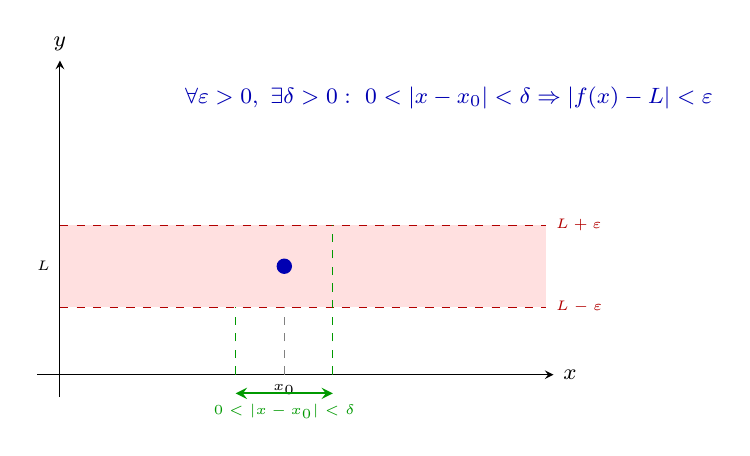
\begin{tikzpicture}[>=stealth, scale=0.95]
    \draw[->] (-0.3,0) -- (6.6,0) node[right, font=\footnotesize] {$x$};
    \draw[->] (0,-0.3) -- (0,4.2) node[above, font=\footnotesize] {$y$};

    \draw[thick, blue!70!black, domain=0.5:5.8, samples=120]
        plot (\x, {1.0 + 0.6*sin(60*\x) + 0.15*\x});

    \def\xz{3.0}
    \pgfmathsetmacro{\yz}{1.0 + 0.6*sin(60*\xz) + 0.15*\xz}

    \draw[dashed, gray] (\xz,0) -- (\xz,\yz);
    \draw[dashed, gray] (0,\yz) -- (\xz,\yz);
    \filldraw[blue!70!black] (\xz,\yz) circle (2.5pt);
    \node[font=\tiny, below] at (\xz,0) {$x_0$};
    \node[font=\tiny, left] at (0,\yz) {$L$};

    \pgfmathsetmacro{\eL}{\yz-0.55}
    \pgfmathsetmacro{\eU}{\yz+0.55}
    \fill[red!12] (0,\eL) rectangle (6.5,\eU);
    \draw[dashed, red!70!black] (0,\eL) -- (6.5,\eL)
        node[right, font=\tiny, red!70!black] {$L-\varepsilon$};
    \draw[dashed, red!70!black] (0,\eU) -- (6.5,\eU)
        node[right, font=\tiny, red!70!black] {$L+\varepsilon$};

    \def\dl{2.35}
    \def\dr{3.65}
    \draw[<->, thick, green!60!black] (\dl,-0.25) -- (\dr,-0.25)
        node[midway, below, font=\tiny, green!60!black]
        {$0<|x-x_0|<\delta$};
    \draw[dashed, green!60!black] (\dl,0) -- (\dl,\eL);
    \draw[dashed, green!60!black] (\dr,0) -- (\dr,\eU);

    \draw[fill=white, thick, blue!70!black] (\xz,\yz) circle (2.5pt);
    \filldraw[blue!70!black] (\xz,\yz) circle (1.5pt);

    \node[font=\footnotesize, blue!70!black, align=center] at (5.2,3.7)
        {$\forall \varepsilon>0,\ \exists \delta>0:\ 0<|x-x_0|<\delta \Rightarrow |f(x)-L|<\varepsilon$};
\end{tikzpicture}
\caption{函数极限的 $\varepsilon$-$\delta$ 可视化。红色横向带为 $(L-\varepsilon,L+\varepsilon)$，绿色区间为对应的 $\delta$-邻域。当 $x$ 落入该邻域（除 $x_0$ 外），$f(x)$ 必落入 $\varepsilon$-带。}
\label{fig:func_limit_epsilon_delta}
\end{figure}

\begin{theorem}[闭区间上连续函数的性质]\label{thm:continuous_closed_interval}
设 $f$ 在闭区间 $[a,b]$ 上连续。则：
\begin{enumerate}[label=(\roman*)]
    \item \textbf{有界性定理}：$f$ 在 $[a,b]$ 上有界。
    \item \textbf{最值定理}：$f$ 在 $[a,b]$ 上必能取到最大值和最小值。
    \item \textbf{介值定理}：若 $f(a) < c < f(b)$，则存在 $\xi \in (a,b)$ 使得 $f(\xi) = c$。
    \item \textbf{一致连续性定理}：$f$ 在 $[a,b]$ 上一致连续。
\end{enumerate}
\end{theorem}

\begin{proof}
\textbf{(i) 有界性定理}：反设 $f$ 在 $[a,b]$ 上无界。则对每个 $n \in \mathbb{N}$，存在 $x_n \in [a,b]$ 使 $|f(x_n)| > n$。由波尔查诺-魏尔斯特拉斯定理（“数系”章实数完备性的推论），有界数列 $\{x_n\}$ 有收敛子列 $\{x_{n_k}\}$，设其极限为 $x_0 \in [a,b]$（因 $[a,b]$ 是闭集）。由 $f$ 的连续性，$\lim_{k\to\infty} f(x_{n_k}) = f(x_0)$。但 $|f(x_{n_k})| > n_k \to \infty$，矛盾。故 $f$ 有界。

\textbf{(ii) 最值定理}：由 (i)，$f$ 在 $[a,b]$ 上有界，故 $M := \sup\{f(x) : x \in [a,b]\}$ 存在。需证存在 $x_0 \in [a,b]$ 使 $f(x_0) = M$。由上确界的定义，对每个 $n$，存在 $x_n \in [a,b]$ 使 $M - 1/n < f(x_n) \le M$。由波尔查诺-魏尔斯特拉斯定理，$\{x_n\}$ 有收敛子列 $\{x_{n_k}\} \to x_0 \in [a,b]$。由连续性，$f(x_0) = \lim_{k} f(x_{n_k}) = M$。最小值同理。

\textbf{(iii) 介值定理}：设 $f(a) < c < f(b)$（$f(a) > c > f(b)$ 的情形类似）。构造集合 $S = \{x \in [a,b] : f(x) < c\}$。$S$ 非空（$a \in S$）且有上界 $b$，故 $\xi := \sup S$ 存在。需证 $f(\xi) = c$。

若 $f(\xi) < c$，则由 $f$ 在 $\xi$ 处的连续性，存在 $\delta > 0$ 使 $(\xi-\delta, \xi+\delta) \cap [a,b]$ 内所有 $x$ 满足 $f(x) < c$。特别地，存在 $x > \xi$ 使 $x \in S$，与 $\xi$ 是 $S$ 的上确界矛盾。

若 $f(\xi) > c$，同理存在 $\delta > 0$ 使 $(\xi-\delta, \xi+\delta) \cap [a,b]$ 内所有 $x$ 满足 $f(x) > c$。这意味着 $\xi - \delta/2$ 是 $S$ 的上界，与 $\xi$ 是最小上界矛盾。

故 $f(\xi) = c$。

\textbf{(iv) 一致连续性定理}：反设 $f$ 在 $[a,b]$ 上不一致连续。则存在 $\varepsilon_0 > 0$，对每个 $n$ 存在 $x_n, y_n \in [a,b]$ 使 $|x_n - y_n| < 1/n$ 但 $|f(x_n) - f(y_n)| \ge \varepsilon_0$。由波尔查诺-魏尔斯特拉斯定理，$\{x_n\}$ 有收敛子列 $\{x_{n_k}\} \to x_0 \in [a,b]$。由于 $|x_{n_k} - y_{n_k}| < 1/n_k \to 0$，$\{y_{n_k}\}$ 也收敛于 $x_0$。由 $f$ 的连续性，$f(x_{n_k}) \to f(x_0)$ 且 $f(y_{n_k}) \to f(x_0)$，故 $|f(x_{n_k}) - f(y_{n_k})| \to 0$，与 $|f(x_{n_k}) - f(y_{n_k})| \ge \varepsilon_0$ 矛盾。
\end{proof}

\begin{figure}[htbp]
\centering
\begin{tikzpicture}[>=stealth, scale=0.9]

    \begin{scope}[shift={(0,0)}]
        \draw[->] (-0.3,0) -- (3.6,0) node[right, font=\tiny] {$x$};
        \draw[->] (0,-0.3) -- (0,2.7) node[above, font=\tiny] {$y$};
        \draw[thick, blue!70!black, domain=0.2:3.4, samples=120]
            plot (\x, {1.3 + 1.1*sin(60*\x) - 0.15*\x});
        \draw[dashed, gray] (0,0.25) -- (3.5,0.25);
        \draw[dashed, gray] (0,2.35) -- (3.5,2.35);
        \node[font=\tiny, left] at (0,2.35) {$M$};
        \node[font=\tiny, left] at (0,0.25) {$m$};
        \filldraw[red!80!black] (1.0,{1.3 + 1.1*sin(60*1.0) - 0.15*1.0}) circle (2.5pt);
        \node[font=\tiny, red!70!black, above] at (1.0,2.2) {最大值点};
        \filldraw[red!80!black] (3.2,{1.3 + 1.1*sin(60*3.2) - 0.15*3.2}) circle (2.5pt);
        \node[font=\tiny, red!70!black, below] at (3.2,0.15) {最小值点};
        \node[font=\small\bfseries, below=0.4cm] at (1.75,-0.9) {(a) 有界性 \& 最值性};
    \end{scope}

    \begin{scope}[shift={(5.5,0)}]
        \draw[->] (-0.3,0) -- (3.6,0) node[right, font=\tiny] {$x$};
        \draw[->] (0,-0.3) -- (0,2.7) node[above, font=\tiny] {$y$};
        \draw[thick, blue!70!black, domain=0.2:3.4, samples=120]
            plot (\x, {0.4 + 1.6*sin(50*\x)});
        \draw[dashed, gray] (0,1.4) -- (3.5,1.4)
            node[right, font=\tiny, gray] {$c$};
        \filldraw[red!80!black] (0.2,{0.4 + 1.6*sin(50*0.2)}) circle (2pt);
        \node[font=\tiny, left] at (0.15,0.7) {$f(a)$};
        \filldraw[red!80!black] (3.4,{0.4 + 1.6*sin(50*3.4)}) circle (2pt);
        \node[font=\tiny, right] at (3.5,1.85) {$f(b)$};
        \filldraw[green!60!black]
            (1.35,{0.4 + 1.6*sin(50*1.35)}) circle (2.5pt);
        \draw[dashed, green!60!black] (1.35,0) -- (1.35,1.4);
        \node[font=\tiny, green!60!black, below] at (1.35,0) {$\xi$};
        \node[font=\small\bfseries, below=0.4cm] at (1.75,-0.9) {(b) 介值定理};
    \end{scope}

    \begin{scope}[shift={(11,0)}]
        \draw[->] (-0.3,0) -- (3.6,0) node[right, font=\tiny] {$x$};
        \draw[->] (0,-0.3) -- (0,2.7) node[above, font=\tiny] {$y$};
        \draw[thick, blue!70!black, domain=0.2:3.4, samples=120]
            plot (\x, {0.8 + 0.9*sin(80*\x)});
        \draw[<->, thick, green!60!black] (1.0,0.15) -- (1.3,0.15)
            node[midway, below, font=\tiny] {$\delta$};
        \draw[<->, thick, red!70!black] (2.5,0.15) -- (2.8,0.15)
            node[midway, below, font=\tiny] {$\delta$};
        \node[font=\tiny, green!60!black] at (1.15,0.9) {变化小};
        \node[font=\tiny, red!70!black] at (2.65,1.5) {变化小};

        \node[font=\footnotesize, align=center] (cnote) at (2.05, 2.30)
            {同一个 $\delta$\\在全区间通用};
        \draw[->, thick, gray!70] (cnote.south) -- (1.85, 1.35);

        \node[font=\small\bfseries, below=0.4cm] at (1.75,-0.9) {(c) 一致连续性};
    \end{scope}
\end{tikzpicture}
\caption{闭区间上连续函数的三个基本性质：(a) 有界性与最值性；(b) 介值定理；(c) 一致连续性。}
\label{fig:closed_interval_continuity}
\end{figure}

\section{\texorpdfstring{导数：函数的方向信息}{导数：函数的方向信息}}

\subsection{\texorpdfstring{导数的定义与求导法则}{导数的定义与求导法则}}

\begin{definition}[导数与极限角]\label{def:derivative}
设函数 $y = f(x)$ 在点 $x_0$ 的某个邻域内有定义。若极限
\[f'(x_0) := \lim_{\Delta x \to 0} \frac{f(x_0 + \Delta x) - f(x_0)}{\Delta x}\]
存在且有限，则称 $f$ 在 $x_0$ 处\textbf{可导}，该极限值称为 $f$ 在 $x_0$ 的\textbf{导数}。导数 $f'(x_0)$ 是一个\textbf{方向量}：其符号指示了函数的变化方向，其绝对值指示了变化速率。

\textbf{极限角}：$f'(x_0) = \tan\theta$，称 $\theta = \arctan(f'(x_0))$ 为 $f$ 在 $x_0$ 处的\textbf{极限角}。极限角是连接向量层面（几何辐角）与函数层面（微积分方向）的核心桥梁。
\end{definition}

\begin{figure}[htbp]
\centering
\begin{tikzpicture}[>=stealth, scale=1.0]
    \draw[->] (-3.2,0) -- (10.2,0) node[right, font=\footnotesize] {$x$};
    \draw[->] (0,-1.4) -- (0,5.4) node[above, font=\footnotesize] {$y$};

    \draw[thick, blue!70!black, domain=0.4:5.2, samples=120]
        plot (\x, {0.5 + 0.35*\x + 0.12*(\x-2.8)*(\x-2.8)});

    \def\xz{2.0}
    \pgfmathsetmacro{\yz}{0.5 + 0.35*\xz + 0.12*(\xz-2.8)*(\xz-2.8)}
    \pgfmathsetmacro{\k}{0.35 + 0.24*(\xz-2.8)}
    \pgfmathsetmacro{\ang}{atan(\k)}

    \draw[thick, red] ({\xz-1.4},{\yz-\k*1.4}) -- ({\xz+2.8},{\yz+\k*2.8});

    \def\dx{1.6}
    \pgfmathsetmacro{\xs}{\xz+\dx}
    \pgfmathsetmacro{\ys}{0.5 + 0.35*\xs + 0.12*(\xs-2.8)*(\xs-2.8)}
    \draw[thick, green!60!black, dashed]
        (\xz,\yz) -- (\xs,\ys);

    \draw[dashed, gray] (\xs,\ys) -- (\xs,\yz) -- (\xz,\yz);

    \filldraw[blue!70!black] (\xz,\yz) circle (2.5pt);
    \filldraw[green!60!black] (\xs,\ys) circle (2pt);

    \draw[thick, orange!80!black] ({\xz+1.4},{\yz}) arc (0:\ang:1.4);
    \draw[dashed, orange!50] ({\xz},{\yz}) -- ({\xz+2.4},{\yz});
    \pgfmathsetmacro{\armx}{\xz+1.5*cos(\ang)}
    \pgfmathsetmacro{\army}{\yz+1.5*sin(\ang)}
    \draw[dashed, orange!50] ({\xz},{\yz}) -- (\armx,\army);

    \node[font=\footnotesize] (labx0) at (0.9,-1.0) {$x_0$};
    \draw[->, thick, blue!70!black] (labx0.north) -- ({\xz-0.05},{\yz-0.15});

    \node[font=\footnotesize] (labxs) at (6.014,4.251) {$x_0+\Delta x$};
    \draw[->, thick, green!60!black] (labxs.south west)
        -- ({\xs+0.08},{\ys+0.10});

    \pgfmathsetmacro{\thx}{\xz+1.65*cos(\ang/2)}
    \pgfmathsetmacro{\thy}{\yz+1.65*sin(\ang/2)}
    \node[font=\footnotesize, orange!80!black] (labth) at (\thx,\thy) {$\theta$};

    \node[font=\footnotesize, red!70!black] (labtan) at (-1.7,3.3)
        {切线斜率 $=f'(x_0)$};
    \draw[->, thick, red!70!black] (labtan.east) -- (1.5,1.20);

    \pgfmathsetmacro{\midx}{\xz+\dx*0.5}
    \pgfmathsetmacro{\midy}{\yz+(\ys-\yz)*0.5}
    \node[font=\footnotesize, green!60!black] (labsec)
        at (\midx, \midy+1.15) {割线斜率 $=\dfrac{\Delta y}{\Delta x}$};
    \draw[->, thick, green!60!black] (labsec.south)
        -- (\midx, \midy+0.08);

    \node[font=\footnotesize, orange!80!black] (labang) at (6.57,1.41)
        {极限角 $\theta=\arctan f'(x_0)$};
    \draw[->, thick, orange!80!black] (labang.west)
        -- (\thx+0.15, \thy-0.08);
\end{tikzpicture}
\caption{导数与极限角的几何解释。割线斜率随 $\Delta x \to 0$ 趋于切线斜率 $f'(x_0)$，而 $f'(x_0)=\tan\theta$，故 $\theta=\arctan f'(x_0)$ 是 $f$ 在 $x_0$ 处的极限角。图中橙色辅助虚线标出 $\theta$ 的两条边：水平方向（$x$ 轴正方向）与切线方向，$\theta$ 即为二者的夹角。}
\label{fig:derivative_limit_angle}
\end{figure}

\begin{proposition}[可导必连续]\label{prop:diff_implies_cont}
若 $f$ 在 $x_0$ 处可导，则 $f$ 在 $x_0$ 处连续。
\end{proposition}

\begin{proof}
\[
\lim_{\Delta x \to 0} [f(x_0+\Delta x) - f(x_0)] = \lim_{\Delta x \to 0} \left( \frac{f(x_0+\Delta x) - f(x_0)}{\Delta x} \cdot \Delta x \right) = f'(x_0) \cdot 0 = 0.
\]
故 $\lim_{\Delta x \to 0} f(x_0+\Delta x) = f(x_0)$，即 $f$ 在 $x_0$ 处连续。
\end{proof}

\begin{theorem}[求导法则]\label{thm:derivative_rules}
设 $u(x)$ 和 $v(x)$ 在 $x$ 处可导，$c$ 为常数。
\begin{enumerate}[label=(\roman*)]
    \item $(c)' = 0$。
    \item $(cu)'(x) = c u'(x)$。
    \item $(u \pm v)'(x) = u'(x) \pm v'(x)$。
    \item $(uv)'(x) = u'(x)v(x) + u(x)v'(x)$。
    \item 若 $v(x) \neq 0$，则 $\left(\frac{u}{v}\right)'(x) = \frac{u'(x)v(x) - u(x)v'(x)}{v(x)^2}$。
\end{enumerate}
\end{theorem}

\begin{proof}
\textbf{(i) 常数}：$\lim_{\Delta x \to 0} \frac{c - c}{\Delta x} = 0$。

\textbf{(ii) 数乘}：$\lim_{\Delta x \to 0} \frac{cu(x+\Delta x) - cu(x)}{\Delta x} = c \lim_{\Delta x \to 0} \frac{u(x+\Delta x) - u(x)}{\Delta x} = cu'(x)$。

\textbf{(iii) 和差}：
\[
\lim_{\Delta x \to 0} \frac{[u(x+\Delta x) \pm v(x+\Delta x)] - [u(x) \pm v(x)]}{\Delta x} = u'(x) \pm v'(x).
\]

\textbf{(iv) 乘积}：
\[
\frac{(uv)(x+\Delta x) - (uv)(x)}{\Delta x} = u(x+\Delta x)\frac{v(x+\Delta x)-v(x)}{\Delta x} + v(x)\frac{u(x+\Delta x)-u(x)}{\Delta x}.
\]
由可导必连续（命题 \ref{prop:diff_implies_cont}），$u(x+\Delta x) \to u(x)$（$\Delta x \to 0$）。取极限得 $(uv)'(x) = u(x)v'(x) + u'(x)v(x)$。

\textbf{(v) 商}：先证 $(1/v)' = -v'/v^2$。由链式法则（定理 \ref{thm:chain_rule}），$(1/v)' = -v'/v^2$（其中 $1/v = v^{-1}$，$(v^{-1})' = -v^{-2}v'$）。再由乘积法则，$(u/v)' = (u \cdot v^{-1})' = u'v^{-1} + u(-v^{-2}v') = (u'v - uv')/v^2$。
\end{proof}

\begin{theorem}[链式法则]\label{thm:chain_rule}
若 $u = g(x)$ 在 $x_0$ 处可导，且 $y = f(u)$ 在 $u_0 = g(x_0)$ 处可导，则
\[(f \circ g)'(x_0) = f'(g(x_0)) \cdot g'(x_0).\]
\end{theorem}

\begin{proof}
由 $f$ 在 $u_0$ 处可导，存在函数 $\eta(\Delta u)$ 满足 $\lim_{\Delta u \to 0} \eta(\Delta u) = 0$，使
\[
f(u_0 + \Delta u) - f(u_0) = f'(u_0)\Delta u + \eta(\Delta u)\Delta u.
\]
令 $\Delta u = g(x_0 + \Delta x) - g(x_0)$。由 $g$ 在 $x_0$ 处可导，$\Delta u = g'(x_0)\Delta x + o(\Delta x)$。代入得
\[
(f \circ g)(x_0 + \Delta x) - (f \circ g)(x_0) = f'(u_0)[g'(x_0)\Delta x + o(\Delta x)] + \eta(\Delta u)\Delta u.
\]
由 $\Delta u \to 0$（$\Delta x \to 0$）且 $\eta(\Delta u) \to 0$，
\[
\lim_{\Delta x \to 0} \frac{(f \circ g)(x_0 + \Delta x) - (f \circ g)(x_0)}{\Delta x} = f'(u_0)g'(x_0).
\]
\end{proof}

\begin{remark}[连续不可导的反例]\label{rem:continuous_not_differentiable}
连续不一定可导。反例：$f(x)=|x|$ 在 $x=0$ 处连续。右导数：
\[
\lim_{h \to 0^+} \frac{|0+h| - |0|}{h} = \lim_{h \to 0^+} \frac{h}{h} = 1.
\]
左导数：
\[
\lim_{h \to 0^-} \frac{|0+h| - |0|}{h} = \lim_{h \to 0^-} \frac{-h}{h} = -1.
\]
左右导数不相等，故 $f$ 在 $x=0$ 处不可导。
\end{remark}

\subsection{\texorpdfstring{微分中值定理}{微分中值定理}}

\begin{theorem}[费马引理]\label{thm:fermat}
若 $f$ 在 $x_0$ 处可导，且在 $x_0$ 处取得局部极值，则 $f'(x_0) = 0$。
\end{theorem}

\begin{proof}
不妨设 $f$ 在 $x_0$ 处取得局部极大值，即存在 $\delta > 0$ 使 $|x - x_0| < \delta$ 时 $f(x) \le f(x_0)$。

当 $\Delta x > 0$（且 $\Delta x < \delta$）时，$f(x_0 + \Delta x) - f(x_0) \le 0$，故
\[
\frac{f(x_0+\Delta x) - f(x_0)}{\Delta x} \le 0.
\]
取极限 $\Delta x \to 0^+$ 得右导数 $f'_+(x_0) \le 0$。

当 $\Delta x < 0$（且 $|\Delta x| < \delta$）时，$f(x_0 + \Delta x) - f(x_0) \le 0$，但 $\Delta x < 0$，故
\[
\frac{f(x_0+\Delta x) - f(x_0)}{\Delta x} \ge 0.
\]
取极限 $\Delta x \to 0^-$ 得左导数 $f'_-(x_0) \ge 0$。

由于 $f$ 可导，$f'_+(x_0) = f'_-(x_0) = f'(x_0)$。因此 $f'(x_0) \le 0$ 且 $f'(x_0) \ge 0$，故 $f'(x_0) = 0$。局部极小值的情形类似。
\end{proof}

\begin{theorem}[罗尔定理]\label{thm:rolle}
若 $f$ 在 $[a,b]$ 上连续，在 $(a,b)$ 内可导，且 $f(a) = f(b)$，则存在 $\xi \in (a,b)$ 使得 $f'(\xi) = 0$。
\end{theorem}

\begin{proof}
由最值定理（定理 \ref{thm:continuous_closed_interval}），$f$ 在 $[a,b]$ 上取得最大值 $M$ 和最小值 $m$。

\textbf{情形 1}：$M = m$。则 $f$ 恒为常数，$f'(x) = 0$ 对所有 $x \in (a,b)$ 成立。

\textbf{情形 2}：$M > m$。由于 $f(a) = f(b)$，最大值和最小值不可能同时在端点取到（若两者都在端点，则 $f(a) = f(b) = M = m$，矛盾）。因此至少有一个极值在 $(a,b)$ 内取到。设 $f(\xi) = M$（或 $m$）且 $\xi \in (a,b)$。由费马引理（定理 \ref{thm:fermat}），$f'(\xi) = 0$。
\end{proof}

\begin{theorem}[拉格朗日中值定理]\label{thm:lagrange}
若 $f$ 在 $[a,b]$ 上连续，在 $(a,b)$ 内可导，则存在 $\xi \in (a,b)$ 使得
\[f(b) - f(a) = f'(\xi)(b-a).\]
\end{theorem}

\begin{proof}
构造辅助函数
\[
\varphi(x) = f(x) - f(a) - \frac{f(b)-f(a)}{b-a}(x-a).
\]
验证 $\varphi$ 满足罗尔定理的条件：(i) $\varphi$ 在 $[a,b]$ 上连续（$f$ 连续减去线性函数）；(ii) $\varphi$ 在 $(a,b)$ 内可导；且
\[
\varphi(a) = f(a) - f(a) - 0 = 0, \qquad
\varphi(b) = f(b) - f(a) - \frac{f(b)-f(a)}{b-a}(b-a) = 0.
\]
由罗尔定理（定理 \ref{thm:rolle}），存在 $\xi \in (a,b)$ 使 $\varphi'(\xi) = 0$。而
\[
\varphi'(x) = f'(x) - \frac{f(b)-f(a)}{b-a}.
\]
代入 $x = \xi$ 即得 $f'(\xi) = \frac{f(b)-f(a)}{b-a}$。
\end{proof}

\begin{corollary}[周期函数的中值性质]\label{cor:periodic_mean_value}
若 $f$ 在 $\mathbb{R}$ 上可导且以 $T$ 为周期，则在一个周期内存在 $\xi \in (x, x+T)$ 使得 $f'(\xi) = 0$。
\end{corollary}

\begin{proof}
对区间 $[x, x+T]$ 应用拉格朗日中值定理（定理 \ref{thm:lagrange}），存在 $\xi \in (x, x+T)$ 使
\[
f(x+T) - f(x) = f'(\xi)T.
\]
由周期性 $f(x+T) = f(x)$，左端为零，故 $f'(\xi)T = 0$，即 $f'(\xi) = 0$。
\end{proof}

\begin{figure}[htbp]
\centering
\begin{tikzpicture}[>=stealth, scale=0.9]

    \begin{scope}[shift={(0,0)}]
        \draw[->] (-0.3,0) -- (3.6,0) node[right, font=\tiny] {$x$};
        \draw[->] (0,-0.3) -- (0,2.6) node[above, font=\tiny] {$y$};
        \draw[thick, blue!70!black, domain=0.3:3.3, samples=120]
            plot (\x, {1.6 - 0.35*(\x-1.8)*(\x-1.8)});
        \draw[dashed, gray] (0,1.02) -- (0.3,1.02);
        \draw[dashed, gray] (0,1.02) -- (3.3,1.02);
        \filldraw[red!80!black] (0.3,1.02) circle (2pt);
        \filldraw[red!80!black] (3.3,1.02) circle (2pt);
        \node[font=\tiny, below] at (0.3,0.95) {$a$};
        \node[font=\tiny, below] at (3.3,0.95) {$b$};
        \filldraw[green!60!black] (1.8,2.0) circle (2.5pt);
        \node[font=\tiny, green!60!black, above] at (1.8,2.05) {$\xi$};
        \draw[thick, red] (1.0,2.0) -- (2.6,2.0);
        \node[font=\small\bfseries, below=0.5cm] at (1.8,-0.95)
            {(a) Rolle：$f'(\xi)=0$};
    \end{scope}

    \begin{scope}[shift={(5.5,0)}]
        \draw[->] (-0.3,0) -- (3.6,0) node[right, font=\tiny] {$x$};
        \draw[->] (0,-0.3) -- (0,2.6) node[above, font=\tiny] {$y$};
        \draw[thick, blue!70!black, domain=0.3:3.3, samples=120]
            plot (\x, {0.5 + 0.35*\x + 0.12*(\x-1.8)*(\x-1.8)});
        \filldraw[red!80!black] (0.3,0.81) circle (2pt);
        \filldraw[red!80!black] (3.3,1.87) circle (2pt);
        \node[font=\tiny, below] at (0.3,0.74) {$a$};
        \node[font=\tiny, below] at (3.3,1.8) {$b$};
        \draw[thick, green!60!black, dashed] (0.3,0.81) -- (3.3,1.87);
        \pgfmathsetmacro{\k}{(1.87-0.81)/(3.3-0.3)}
        \draw[thick, red] (1.1,1.55) -- (2.5,1.55+\k*1.4);
        \filldraw[green!60!black] (1.8,1.55+\k*0.7) circle (2.5pt);
        \node[font=\tiny, green!60!black, below] at (1.8,1.55+\k*0.7) {$\xi$};
        \node[font=\small\bfseries, below=0.5cm] at (1.8,-0.95)
            {(b) Lagrange：$f'(\xi)=\frac{f(b)-f(a)}{b-a}$};
    \end{scope}

    \begin{scope}[shift={(11,0)}]
        \draw[->] (-0.3,0) -- (3.6,0) node[right, font=\tiny] {$x$};
        \draw[->] (0,-0.3) -- (0,2.6) node[above, font=\tiny] {$y$};
        \draw[thick, blue!70!black, domain=0.3:3.3, samples=100]
            plot ({\x},{1.6 - 0.35*(\x-1.8)*(\x-1.8)});
        \draw[thick, orange!80!black, domain=0.3:3.3, samples=100]
            plot ({\x},{0.3 + 0.4*\x});
        \filldraw[red!80!black] (0.3,{1.6 - 0.35*(0.3-1.8)*(0.3-1.8)}) circle (2pt);
        \filldraw[red!80!black] (3.3,{1.6 - 0.35*(3.3-1.8)*(3.3-1.8)}) circle (2pt);
        \filldraw[orange!80!black] (0.3,{0.3+0.4*0.3}) circle (2pt);
        \filldraw[orange!80!black] (3.3,{0.3+0.4*3.3}) circle (2pt);
        \draw[thick, green!60!black, dashed]
            (1.6,0.5) -- (2.0,2.0);
        \filldraw[green!60!black] (1.8,1.25) circle (2.5pt);
        \node[font=\tiny, green!60!black, right] at (1.85,1.25) {$\xi$};
        \node[font=\small\bfseries, below=0.5cm] at (1.8,-0.95)
            {(c) Cauchy：$\frac{f'(\xi)}{g'(\xi)}=\frac{f(b)-f(a)}{g(b)-g(a)}$};
    \end{scope}
\end{tikzpicture}
\caption{三大中值定理的几何图像：(a) 罗尔定理；(b) 拉格朗日中值定理；(c) 柯西中值定理。虚线为割线，实线为对应的平行切线。}
\label{fig:mean_value_theorems}
\end{figure}

\subsection{\texorpdfstring{高阶导数与偏导数}{高阶导数与偏导数}}

\begin{proposition}[高阶导数的方向意义]\label{prop:higher_derivative_direction}
设 $f$ 在点 $x_0$ 处 $n$ 阶可导。
\begin{enumerate}[label=(\roman*)]
    \item \textbf{一阶导数} $f'(x_0)$：切线方向，极限角 $\theta^{(1)} = \arctan(f'(x_0))$。
    \item \textbf{二阶导数} $f''(x_0)$：凹凸方向，极限角 $\theta^{(2)} = \arctan(f''(x_0))$。
    \item \textbf{$n$ 阶导数} $f^{(n)}(x_0)$：更精细的弯曲方向。
\end{enumerate}
\end{proposition}

\begin{proof}
(i) 由定义 \ref{def:derivative} 直接得出：$f'(x_0) = \tan\theta^{(1)}$，$\theta^{(1)} = \arctan(f'(x_0))$。

(ii) $f''(x_0) = (f')'(x_0)$ 是导函数 $f'$ 在 $x_0$ 处的导数。由导数的定义，$f''(x_0)$ 的符号决定 $f'$ 的单调性：$f''(x_0) > 0$ 意味着 $f'$ 在 $x_0$ 附近递增（函数上凹），$f''(x_0) < 0$ 意味着 $f'$ 在 $x_0$ 附近递减（函数下凹）。极限角 $\theta^{(2)} = \arctan(f''(x_0))$ 度量了“凹凸方向”的倾斜程度。

(iii) 由数学归纳法：$f^{(n)}(x_0) = (f^{(n-1)})'(x_0)$ 是第 $n-1$ 阶导函数在 $x_0$ 处的导数，刻画了第 $n-1$ 阶方向的变化率，即“更精细的弯曲方向”。
\end{proof}

\begin{definition}[偏导数作为单方向算子]\label{def:partial_derivative}
设二元函数 $u = f(x, y)$ 在点 $(x_0, y_0)$ 的邻域内有定义。若极限
\[\frac{\partial f}{\partial x}(x_0, y_0) := \lim_{\Delta x \to 0} \frac{f(x_0 + \Delta x, y_0) - f(x_0, y_0)}{\Delta x}\]
存在且有限，则称 $f$ 在 $(x_0, y_0)$ 处对 $x$ \textbf{可偏导}。类似地可定义 $\frac{\partial f}{\partial y}$。

偏导数 $\frac{\partial f}{\partial x}$ 是曲面 $z = f(x,y)$ 与平面 $y = y_0$ 相交所得曲线在 $x_0$ 处的切线斜率。
\end{definition}

\begin{definition}[全微分与方向增量]\label{def:total_differential}
若 $f(x, y)$ 在 $(x_0, y_0)$ 处的全增量可表示为
\[\Delta f = A\Delta x + B\Delta y + o\!\left(\sqrt{\Delta x^2 + \Delta y^2}\right),\]
则称 $f$ 在 $(x_0, y_0)$ 处\textbf{可微}，$df = A\,dx + B\,dy$ 为\textbf{全微分}。此时必有 $A = \frac{\partial f}{\partial x}$，$B = \frac{\partial f}{\partial y}$。
\end{definition}

\begin{definition}[梯度作为方向导数最大值方向]\label{def:gradient_direction}
函数 $f(x, y)$ 在点 $(x_0, y_0)$ 处的\textbf{梯度}为
\[\nabla f(x_0, y_0) = \left( \frac{\partial f}{\partial x}, \frac{\partial f}{\partial y} \right).\]
梯度方向是方向导数取最大值的方向，其模长等于最大变化率。
\end{definition}

\begin{definition}[高阶偏导数与混合偏导数]\label{def:higher_partial}
若偏导数 $\frac{\partial f}{\partial x}$ 仍可偏导，则称
\[\frac{\partial^2 f}{\partial x^2} = \frac{\partial}{\partial x}\left(\frac{\partial f}{\partial x}\right),\quad
\frac{\partial^2 f}{\partial y \partial x} = \frac{\partial}{\partial y}\left(\frac{\partial f}{\partial x}\right)\]
为二阶偏导数。
\end{definition}

\begin{proposition}[可微与偏导的关系]\label{prop:diff_partial}
若 $f$ 在 $(x_0, y_0)$ 处可微，则两个一阶偏导数均存在。反之，偏导数存在不能保证可微。
\end{proposition}

\begin{proof}
\textbf{正方向}：设 $f$ 在 $(x_0, y_0)$ 处可微，则
\[
\Delta f = A\Delta x + B\Delta y + o\!\left(\sqrt{\Delta x^2 + \Delta y^2}\right).
\]
取 $\Delta y = 0$，则
\[
f(x_0 + \Delta x, y_0) - f(x_0, y_0) = A\Delta x + o(|\Delta x|).
\]
除以 $\Delta x$ 并取极限：
\[
\frac{\partial f}{\partial x}(x_0, y_0) = \lim_{\Delta x \to 0} \frac{f(x_0+\Delta x, y_0) - f(x_0, y_0)}{\Delta x} = A.
\]
同理 $\frac{\partial f}{\partial y}(x_0, y_0) = B$。

\textbf{反方向（反例）}：见注 \ref{rem:partial_not_differentiable}。
\end{proof}

\begin{lemma}[方向导数的存在性]\label{lem:directional_derivative}
若 $f$ 在 $(x_0, y_0)$ 处可微，则对任意单位方向向量 $\boldsymbol{l} = (\cos\alpha, \cos\beta)$，方向导数
\[\frac{\partial f}{\partial \boldsymbol{l}} = \nabla f \cdot \boldsymbol{l} = f_x \cos\alpha + f_y \cos\beta\]
存在。
\end{lemma}

\begin{proof}
由全微分的定义（定义 \ref{def:total_differential}），
\[
f(x_0 + t\cos\alpha, y_0 + t\cos\beta) - f(x_0, y_0) = f_x(x_0,y_0)\,t\cos\alpha + f_y(x_0,y_0)\,t\cos\beta + o(t).
\]
除以 $t$ 并令 $t \to 0$：
\[
\frac{\partial f}{\partial \boldsymbol{l}}(x_0, y_0) = \lim_{t \to 0} \frac{f(x_0 + t\cos\alpha, y_0 + t\cos\beta) - f(x_0, y_0)}{t} = f_x \cos\alpha + f_y \cos\beta = \nabla f \cdot \boldsymbol{l}.
\]
\end{proof}

\begin{theorem}[多元链式法则]\label{thm:multivariable_chain_rule}
设 $u = f(x, y)$ 可微，$x = x(t), y = y(t)$ 可导，则
\[\frac{du}{dt} = \frac{\partial f}{\partial x}\frac{dx}{dt} + \frac{\partial f}{\partial y}\frac{dy}{dt}.\]
\end{theorem}

\begin{proof}
由 $f$ 可微，
\[
\Delta f = \frac{\partial f}{\partial x}\Delta x + \frac{\partial f}{\partial y}\Delta y + o\!\left(\sqrt{\Delta x^2 + \Delta y^2}\right).
\]
由 $x(t), y(t)$ 可导，
\[
\Delta x = x'(t)\Delta t + o(\Delta t), \qquad \Delta y = y'(t)\Delta t + o(\Delta t).
\]
代入得
\[
\Delta f = \left( \frac{\partial f}{\partial x}x'(t) + \frac{\partial f}{\partial y}y'(t) \right)\Delta t + o(\Delta t).
\]
除以 $\Delta t$ 并取极限即得。
\end{proof}

\begin{theorem}[混合偏导数相等（Clairaut 定理）]\label{thm:clairaut}
若 $f_{xy}$ 与 $f_{yx}$ 在点 $(x_0, y_0)$ 的邻域内连续，则
\[\frac{\partial^2 f}{\partial x \partial y}(x_0, y_0) = \frac{\partial^2 f}{\partial y \partial x}(x_0, y_0).\]
\end{theorem}

\begin{proof}
考虑二阶差分
\[
\Delta(h,k) = f(x_0+h, y_0+k) - f(x_0+h, y_0) - f(x_0, y_0+k) + f(x_0, y_0).
\]
定义 $\varphi(x) = f(x, y_0+k) - f(x, y_0)$。则
\[
\Delta(h,k) = \varphi(x_0+h) - \varphi(x_0).
\]
由拉格朗日中值定理，存在 $\xi$ 介于 $x_0$ 与 $x_0+h$ 之间，使
\[
\Delta(h,k) = h\varphi'(\xi) = h[f_x(\xi, y_0+k) - f_x(\xi, y_0)].
\]
再对 $y$ 应用中值定理，存在 $\eta$ 介于 $y_0$ 与 $y_0+k$ 之间，使
\[
\Delta(h,k) = hk\, f_{xy}(\xi, \eta).
\]
类似地，定义 $\psi(y) = f(x_0+h, y) - f(x_0, y)$，则
\[
\Delta(h,k) = \psi(y_0+k) - \psi(y_0) = k\psi'(\eta') = k[f_y(x_0+h, \eta') - f_y(x_0, \eta')] = hk\, f_{yx}(\xi', \eta').
\]
故
\[
f_{xy}(\xi, \eta) = f_{yx}(\xi', \eta').
\]
令 $(h,k) \to (0,0)$，则 $(\xi,\eta) \to (x_0,y_0)$ 且 $(\xi',\eta') \to (x_0,y_0)$。由 $f_{xy}$ 和 $f_{yx}$ 的连续性，
\[
f_{xy}(x_0,y_0) = f_{yx}(x_0,y_0).
\]
\end{proof}

\begin{remark}[偏导存在不可微的反例]\label{rem:partial_not_differentiable}
$f(x,y) = \frac{xy}{x^2+y^2}$（$f(0,0)=0$）。在 $(0,0)$ 处：
\[
\frac{\partial f}{\partial x}(0,0) = \lim_{\Delta x \to 0} \frac{f(\Delta x, 0) - f(0,0)}{\Delta x} = \lim_{\Delta x \to 0} \frac{0 - 0}{\Delta x} = 0,
\]
同理 $\frac{\partial f}{\partial y}(0,0) = 0$。但沿直线 $y = kx$ 的极限为
\[
\lim_{x \to 0} f(x, kx) = \lim_{x \to 0} \frac{kx^2}{x^2 + k^2x^2} = \frac{k}{1+k^2},
\]
随 $k$ 变化，故 $f$ 在 $(0,0)$ 处不连续，更不可微。
\end{remark}

\section{\texorpdfstring{微分：函数的线性逼近}{微分：函数的线性逼近}}

\begin{definition}[微分作为方向增量的线性主部]\label{def:differential}
设 $y = f(x)$ 在 $x_0$ 处可导。若增量
\[\Delta y = f(x_0 + \Delta x) - f(x_0) = f'(x_0)\,\Delta x + o(\Delta x) \quad (\Delta x \to 0),\]
则称 $dy := f'(x_0)\,dx$ 为 $f$ 在 $x_0$ 处的\textbf{微分}。
\end{definition}

\begin{lemma}[微分运算与导数运算的一致性]\label{lem:differential_rules}
设 $u(x), v(x)$ 在 $x$ 处可微，$c$ 为常数，则
\begin{enumerate}[label=(\roman*)]
    \item $d(c) = 0$；
    \item $d(cu) = c\,du$；
    \item $d(u \pm v) = du \pm dv$；
    \item $d(uv) = v\,du + u\,dv$；
    \item $d\!\left(\frac{u}{v}\right) = \frac{v\,du - u\,dv}{v^2}\;(v \neq 0)$。
\end{enumerate}
\end{lemma}

\begin{proof}
(i) $d(c) = c'\,dx = 0 \cdot dx = 0$。

(ii) $d(cu) = (cu)'\,dx = cu'\,dx = c\,du$。

(iii) $d(u \pm v) = (u \pm v)'\,dx = (u' \pm v')\,dx = du \pm dv$。

(iv) $d(uv) = (uv)'\,dx = (u'v + uv')\,dx = v(u'\,dx) + u(v'\,dx) = v\,du + u\,dv$。

(v) $d(u/v) = (u/v)'\,dx = \frac{u'v - uv'}{v^2}\,dx = \frac{v(u'\,dx) - u(v'\,dx)}{v^2} = \frac{v\,du - u\,dv}{v^2}$。

以上每一步都由求导法则（定理 \ref{thm:derivative_rules}）直接得出。
\end{proof}

\begin{theorem}[一阶微分形式不变性]\label{thm:invariance_differential}
设 $y = f(u)$ 可微，$u = g(x)$ 可微，则 $dy = f'(u)\,du = f'(g(x))\,g'(x)\,dx$。
\end{theorem}

\begin{proof}
由链式法则（定理 \ref{thm:chain_rule}），$(f \circ g)'(x) = f'(g(x))\,g'(x)$。因此
\[
dy = (f \circ g)'(x)\,dx = f'(g(x))\,g'(x)\,dx.
\]
另一方面，$du = g'(x)\,dx$，故 $f'(u)\,du = f'(g(x))\,g'(x)\,dx$。两者相等。
\end{proof}

\begin{corollary}[微分的线性逼近性质]\label{cor:linear_approximation}
若 $f$ 在 $x_0$ 处可微，则当 $|x - x_0|$ 充分小时，
\[f(x) \approx f(x_0) + f'(x_0)(x - x_0).\]
\end{corollary}

\begin{proof}
由微分的定义（定义 \ref{def:differential}），
\[
f(x) - f(x_0) = f'(x_0)(x - x_0) + o(|x - x_0|).
\]
当 $|x - x_0| \to 0$ 时，$o(|x-x_0|)$ 比 $|x-x_0|$ 更快地趋于零，故
\[
f(x) = f(x_0) + f'(x_0)(x - x_0) + o(|x - x_0|) \approx f(x_0) + f'(x_0)(x - x_0).
\]
\end{proof}

\section{\texorpdfstring{积分：函数的趋势信息}{积分：函数的趋势信息}}

\subsection{\texorpdfstring{一元积分}{一元积分}}

\begin{definition}[不定积分作为方向的逆运算]\label{def:indefinite_integral}
设 $f$ 在区间 $I$ 上连续。若存在可微函数 $F$，使得 $F'(x) = f(x)$ 对所有 $x \in I$ 成立，则称 $F$ 为 $f$ 的一个\textbf{原函数}。$f$ 的全体原函数称为\textbf{不定积分}，记作
\[\int f(x)\,dx = F(x) + C.\]
\end{definition}

\begin{definition}[黎曼积分]\label{def:riemann_integral}
设 $f$ 在 $[a,b]$ 上有界。对分割 $\mathcal{P}: a = x_0 < x_1 < \cdots < x_n = b$，任取 $\xi_i \in [x_{i-1}, x_i]$，构造黎曼和
\[S(f, \mathcal{P}, \{\xi_i\}) = \sum_{i=1}^{n} f(\xi_i)\,\Delta x_i.\]
若当 $\|\mathcal{P}\| \to 0$ 时极限存在且与分割及取点方式无关，则称 $f$ 在 $[a,b]$ 上\textbf{黎曼可积}，极限值称为\textbf{定积分}，记作 $\int_a^b f(x)\,dx$。
\end{definition}

\begin{theorem}[微积分基本定理——方向与趋势的对偶]\label{thm:ftc}
设 $f$ 在 $[a,b]$ 上连续。
\begin{enumerate}[label=(\roman*)]
    \item 变上限积分 $\Phi(x) = \int_a^x f(t)\,dt$ 在 $[a,b]$ 上可导，且 $\Phi'(x) = f(x)$。
    \item 若 $F$ 是 $f$ 的任意一个原函数，则 $\int_a^b f(x)\,dx = F(b) - F(a)$。
\end{enumerate}
\end{theorem}

\begin{proof}
\textbf{(i)} 对 $\Delta x > 0$（$\Delta x < 0$ 类似），
\[
\frac{\Phi(x+\Delta x) - \Phi(x)}{\Delta x} = \frac{1}{\Delta x}\int_x^{x+\Delta x} f(t)\,dt.
\]
由连续函数在闭区间上的最值定理，$f$ 在 $[x, x+\Delta x]$ 上取得最小值 $m(\Delta x)$ 和最大值 $M(\Delta x)$，故
\[
m(\Delta x) \le \frac{1}{\Delta x}\int_x^{x+\Delta x} f(t)\,dt \le M(\Delta x).
\]
当 $\Delta x \to 0^+$ 时，由 $f$ 的连续性，$m(\Delta x) \to f(x)$ 且 $M(\Delta x) \to f(x)$。由夹逼定理，
\[
\lim_{\Delta x \to 0^+} \frac{\Phi(x+\Delta x) - \Phi(x)}{\Delta x} = f(x).
\]
同理左导数也为 $f(x)$。故 $\Phi'(x) = f(x)$。

\textbf{(ii)} 令 $G(x) = \Phi(x) - F(x)$。由 (i)，$G'(x) = \Phi'(x) - F'(x) = f(x) - f(x) = 0$。由拉格朗日中值定理的推论（导数为零的函数是常数），$G$ 在 $[a,b]$ 上为常数。因此
\[
\Phi(b) - F(b) = G(b) = G(a) = \Phi(a) - F(a) = -F(a).
\]
故 $\Phi(b) = F(b) - F(a)$，即 $\int_a^b f(x)\,dx = F(b) - F(a)$。
\end{proof}

\begin{corollary}[微分与积分的互逆性]\label{cor:diff_int_inverse}
若 $f$ 连续，则
\[\frac{d}{dx}\left( \int_a^x f(t)\,dt \right) = f(x),\qquad
\int_a^b F'(x)\,dx = F(b) - F(a).\]
\end{corollary}

\begin{proof}
第一式由定理 \ref{thm:ftc} (i) 直接给出。第二式由定理 \ref{thm:ftc} (ii) 应用于 $F' = f$ 直接给出。
\end{proof}

\begin{figure}[htbp]
\centering
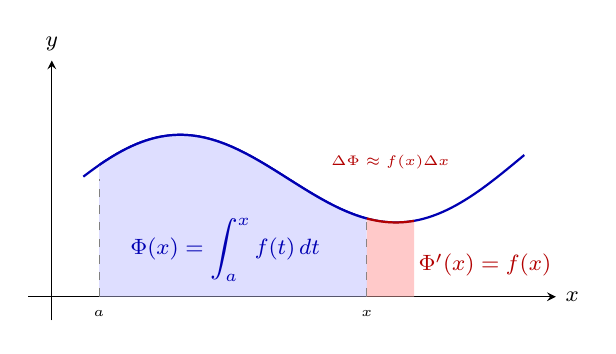
\begin{tikzpicture}[>=stealth, scale=1.0]
    \draw[->] (-0.3,0) -- (6.4,0) node[right, font=\footnotesize] {$x$};
    \draw[->] (0,-0.3) -- (0,3.0) node[above, font=\footnotesize] {$y$};

    \draw[thick, blue!70!black, domain=0.4:6.0, samples=120]
        plot (\x, {1.2 + 0.7*sin(60*\x) + 0.10*\x});

    \def\a{0.6}
    \def\xz{4.0}
    \fill[blue!20, opacity=0.65]
        ({\a},0) -- plot[domain=\a:\xz, samples=100]
        (\x, {1.2 + 0.7*sin(60*\x) + 0.10*\x}) -- (\xz,0) -- cycle;
    \draw[thick, blue!70!black, domain=\a:\xz, samples=100]
        plot (\x, {1.2 + 0.7*sin(60*\x) + 0.10*\x});
    \draw[dashed, gray] (\a,0) -- (\a,1.5);
    \draw[dashed, gray] (\xz,0) -- (\xz,{1.2 + 0.7*sin(60*\xz) + 0.10*\xz});
    \node[font=\tiny, below] at (\a,-0.05) {$a$};
    \node[font=\tiny, below] at (\xz,-0.05) {$x$};

    \node[font=\footnotesize, blue!70!black] at (2.2,0.6)
        {$\Phi(x)=\displaystyle\int_a^x f(t)\,dt$};

    \def\dx{0.6}
    \pgfmathsetmacro{\xu}{\xz+\dx}
    \pgfmathsetmacro{\hu}{1.2 + 0.7*sin(60*\xu) + 0.10*\xu}
    \fill[red!30, opacity=0.7]
        (\xz,0) -- plot[domain=\xz:\xu, samples=40]
        (\x, {1.2 + 0.7*sin(60*\x) + 0.10*\x}) -- (\xu,0) -- cycle;
    \draw[thick, red!70!black, domain=\xz:\xu, samples=40]
        plot (\x, {1.2 + 0.7*sin(60*\x) + 0.10*\x});
    \node[font=\tiny, red!70!black, above] at (\xz+0.3,1.5)
        {$\Delta\Phi\approx f(x)\Delta x$};

    \node[font=\footnotesize, red!70!black] at (5.5,0.4)
        {$\Phi'(x)=f(x)$};
\end{tikzpicture}
\caption{微积分基本定理的几何图像。变上限积分 $\Phi(x)$ 是曲线下的面积，其增量 $\Delta\Phi \approx f(x)\Delta x$——这是 $\Phi'(x)=f(x)$ 的几何含义。}
\label{fig:ftc_area}
\end{figure}

\begin{property}[定积分的基本性质]\label{prop:integral_properties}
设 $f, g$ 在 $[a,b]$ 上可积，$c \in [a,b]$。则：
\begin{enumerate}[label=(\roman*)]
    \item \textbf{线性性}：$\int_a^b (f + cg)\,dx = \int_a^b f\,dx + c\int_a^b g\,dx$；
    \item \textbf{区间可加性}：$\int_a^b f\,dx = \int_a^c f\,dx + \int_c^b f\,dx$；
    \item \textbf{保序性}：若 $f \le g$，则 $\int_a^b f\,dx \le \int_a^b g\,dx$；
    \item \textbf{绝对值估计}：$\left|\int_a^b f\,dx\right| \le \int_a^b |f|\,dx$。
\end{enumerate}
\end{property}

\begin{proof}
(i) 由黎曼和的线性性与极限的线性性：
\[
\int_a^b (f+cg) = \lim \sum (f(\xi_i) + cg(\xi_i))\Delta x_i = \lim \sum f(\xi_i)\Delta x_i + c\lim \sum g(\xi_i)\Delta x_i.
\]

(ii) 任何 $[a,b]$ 的分割可以加入 $c$ 作为分点，$\int_a^b f = \int_a^c f + \int_c^b f$ 由黎曼和的可加性直接得出。

(iii) 若 $f \le g$，则对任意黎曼和，$\sum f(\xi_i)\Delta x_i \le \sum g(\xi_i)\Delta x_i$。取极限即得。

(iv) 由 $-|f| \le f \le |f|$ 和 (iii)，
\[
-\int_a^b |f|\,dx \le \int_a^b f\,dx \le \int_a^b |f|\,dx,
\]
即 $\left|\int_a^b f\,dx\right| \le \int_a^b |f|\,dx$。
\end{proof}

\subsection{\texorpdfstring{多元积分}{多元积分}}

\begin{definition}[二重积分]\label{def:double_integral}
设 $f(x,y)$ 在有界闭区域 $D \subset \mathbb{R}^2$ 上有界。将 $D$ 分割为 $n$ 个子区域 $\Delta D_i$，任取 $(\xi_i, \eta_i) \in \Delta D_i$，构造黎曼和
\[S = \sum_{i=1}^n f(\xi_i, \eta_i)\,\Delta A_i.\]
若极限存在，则称 $f$ 在 $D$ 上\textbf{可积}，极限称为\textbf{二重积分}：
\[\iint_D f(x,y)\,dA = \lim_{\|\mathcal{P}\| \to 0} \sum_{i=1}^n f(\xi_i, \eta_i)\,\Delta A_i.\]
\end{definition}

\begin{definition}[三重积分]\label{def:triple_integral}
设 $\Omega \subseteq \mathbb{R}^3$ 为空间区域。$f$ 在 $\Omega$ 上的\textbf{三重积分}定义为
\[\iiint_\Omega f(x, y, z)\,dV.\]
三重积分是三维趋势累积。
\end{definition}

\begin{lemma}[积分中值定理]\label{lem:integral_mean_value}
若 $f$ 在有界闭区域 $D$ 上连续，则存在 $(\xi, \eta) \in D$，使得
\[\iint_D f(x,y)\,dA = f(\xi, \eta) \cdot \mathrm{Area}(D).\]
\end{lemma}

\begin{proof}
由最值定理，$f$ 在 $D$ 上取得最小值 $m$ 和最大值 $M$。则
\[
m \cdot \mathrm{Area}(D) \le \iint_D f(x,y)\,dA \le M \cdot \mathrm{Area}(D).
\]
故
\[
m \le \frac{\iint_D f(x,y)\,dA}{\mathrm{Area}(D)} \le M.
\]
由介值定理（$D$ 是连通集，$f(D)$ 是区间），存在 $(\xi, \eta) \in D$ 使
\[
f(\xi, \eta) = \frac{\iint_D f(x,y)\,dA}{\mathrm{Area}(D)}.
\]
\end{proof}

\begin{theorem}[Fubini 定理——累次积分与方向分解]\label{thm:fubini}
若 $f(x,y)$ 在矩形区域 $D = [a,b] \times [c,d]$ 上连续，则
\[\iint_D f(x,y)\,dA = \int_a^b \left( \int_c^d f(x,y)\,dy \right) dx = \int_c^d \left( \int_a^b f(x,y)\,dx \right) dy.\]
\end{theorem}

\begin{proof}
我们证明第一个等式（第二个同理）。

\textbf{步骤 1}：定义 $F(x) = \int_c^d f(x,y)\,dy$。需证 $F$ 在 $[a,b]$ 上连续。

对任意 $x_1, x_2 \in [a,b]$，
\[
|F(x_1) - F(x_2)| \le \int_c^d |f(x_1,y) - f(x_2,y)|\,dy.
\]
由 $f$ 在有界闭矩形上的一致连续性（定理 \ref{thm:continuous_closed_interval} 的多变量版本），对任意 $\varepsilon > 0$，存在 $\delta > 0$ 使 $|x_1 - x_2| < \delta$ 时 $|f(x_1,y) - f(x_2,y)| < \varepsilon/(d-c)$ 对所有 $y \in [c,d]$ 成立。故 $|F(x_1) - F(x_2)| < \varepsilon$，$F$ 一致连续。

\textbf{步骤 2}：证明 $\iint_D f = \int_a^b F(x)\,dx$。

将 $[a,b]$ 分割为 $m$ 等份，$[c,d]$ 分割为 $n$ 等份，得网格分割 $\mathcal{P}$。设 $m_{ij} = \inf\{f(x,y) : x \in [x_{i-1}, x_i], y \in [y_{j-1}, y_j]\}$，$M_{ij} = \sup\{f(x,y) : x \in [x_{i-1}, x_i], y \in [y_{j-1}, y_j]\}$。

下和与上和分别为
\[
L(\mathcal{P}) = \sum_{i,j} m_{ij}\Delta x_i \Delta y_j, \qquad U(\mathcal{P}) = \sum_{i,j} M_{ij}\Delta x_i \Delta y_j.
\]
对每个固定的 $x \in [x_{i-1}, x_i]$，
\[
\sum_j m_{ij}\Delta y_j \le \int_c^d f(x,y)\,dy = F(x) \le \sum_j M_{ij}\Delta y_j.
\]
在 $[x_{i-1}, x_i]$ 上对 $x$ 积分：
\[
\sum_j m_{ij}\Delta y_j \cdot \Delta x_i \le \int_{x_{i-1}}^{x_i} F(x)\,dx \le \sum_j M_{ij}\Delta y_j \cdot \Delta x_i.
\]
对 $i$ 求和：
\[
L(\mathcal{P}) \le \int_a^b F(x)\,dx \le U(\mathcal{P}).
\]
由 $f$ 可积，$\lim_{\|\mathcal{P}\|\to 0} L(\mathcal{P}) = \lim_{\|\mathcal{P}\|\to 0} U(\mathcal{P}) = \iint_D f$。由夹逼定理，
\[
\int_a^b F(x)\,dx = \iint_D f(x,y)\,dA.
\]
\end{proof}

\begin{proposition}[多重积分的变量代换]\label{prop:change_of_variables}
设 $\mathbf{T}: D^* \to D$ 是双射变换，$(u, v) \mapsto (x(u,v), y(u,v))$。则
\[\iint_D f(x, y)\,dA = \iint_{D^*} f(x(u,v), y(u,v)) \left|\frac{\partial(x, y)}{\partial(u, v)}\right|\,du\,dv,\]
其中 $\frac{\partial(x, y)}{\partial(u, v)}$ 是 Jacobi 行列式，度量了变换的局部面积缩放因子。
\end{proposition}

\begin{proof}
将 $D^*$ 分割为小矩形 $[u_i, u_i+\Delta u] \times [v_j, v_j+\Delta v]$。在 $\mathbf{T}$ 下，该小矩形近似映射为 $D$ 中的平行四边形，其两边为
\[
\mathbf{T}(u_i+\Delta u, v_j) - \mathbf{T}(u_i, v_j) \approx \frac{\partial \mathbf{T}}{\partial u}\Delta u, \qquad
\mathbf{T}(u_i, v_j+\Delta v) - \mathbf{T}(u_i, v_j) \approx \frac{\partial \mathbf{T}}{\partial v}\Delta v.
\]
该平行四边形的面积为
\[
\left\|\frac{\partial \mathbf{T}}{\partial u} \times \frac{\partial \mathbf{T}}{\partial v}\right\| \Delta u \Delta v = \left|\frac{\partial(x,y)}{\partial(u,v)}\right| \Delta u \Delta v.
\]
因此黎曼和满足
\[
\sum f(x_i, y_j)\Delta A_{ij} \approx \sum f(\mathbf{T}(u_i, v_j)) \left|\frac{\partial(x,y)}{\partial(u,v)}\right| \Delta u \Delta v.
\]
取极限即得变量代换公式。
\end{proof}

\begin{example}[球坐标下的三重积分]\label{ex:spherical_coordinates}
在球坐标 $(r, \theta, \phi)$ 下，体积微元为 $dV = r^2 \sin\theta \, dr\, d\theta\, d\phi$。$r^2$ 因子是平方反比定律在积分测度中的体现。
\end{example}

\section{\texorpdfstring{极限角与微分相似度}{极限角与微分相似度}}

\begin{figure}[htbp]
\centering
\begin{tikzpicture}[scale=1.25,>=stealth]
    \draw[->] (-0.5,0) -- (3.5,0) node[right] {\footnotesize $x$};
    \draw[->] (0,-0.5) -- (0,2.9) node[above] {\footnotesize $y$};
    \draw[gray!60] (0,0) circle (2.4);
    \draw[->,thick,blue] (0,0) -- (2.4,0) node[below right] {\footnotesize $\mathbf b$};
    \draw[->,thick,red] (0,0) -- (60:2.4) node[above right] {\footnotesize $\mathbf a$};
    \draw[->,gray] (0.8,0) arc (0:60:0.8);
    \node[font=\footnotesize] at (1.02,0.45) {$\theta$};
    \draw[dashed,gray] (60:2.4) -- (1.2,0);
    \draw[<->,gray] (1.2,0) -- (1.2,2.078);
    \node[font=\footnotesize,blue] at (1.85,-0.30) {$\|\mathbf a\|\cos\theta$};
    \node[font=\footnotesize,red] at (2.25,1.45) {$\|\mathbf a\|\sin\theta$};
    \node[font=\footnotesize] at (2.6,-0.75) {（沿 $\mathbf b$ 分解）};
\end{tikzpicture}
\caption{极限角与沿向分解。把 $\mathbf a$ 沿 $\mathbf b$ 的方向作正交分解：沿向分量 $\|\mathbf a\|\cos\theta$ 度量\textbf{方向的一致程度}（余弦族），垂向分量 $\|\mathbf a\|\sin\theta$ 度量\textbf{方向的偏离程度}（正弦族）。两者的归一化版本 $\cos\theta$、$\sin\theta$ 即本章的极限角；未归一化版本（再乘 $\|\mathbf b\|$）对应后面各章的“趋势”。}
\label{fig:limit_angle_decomposition}
\end{figure}

\begin{definition}[极限角]\label{def:limit_angle}
设函数 $f$ 在点 $a$ 处可导。$f$ 在 $a$ 处的\textbf{极限角}定义为
\[\theta_f(a) = \arctan(f'(a)).\]
极限角是连接向量层面（几何辐角）与函数层面（微积分方向）的核心桥梁。

\textbf{导数辐角}：对可导函数 $f$，当 $f'(a) \neq 0$ 时，称 $\arg f'(a)$ 为 $f$ 在 $a$ 处的\textbf{导数辐角}；它在模 $2\pi$ 的意义下确定，记作 $\arg f'(a) \in \mathbb{R}/2\pi\mathbb{Z}$。实值函数在实变量处的极限角 $\theta_f(a) = \arctan(f'(a))$ 恰是导数辐角落在主值区间 $(-\pi/2, \pi/2)$ 内的那个代表元；复值函数的导数辐角一般不再有这种实代表元，故凡涉及复值情形，一律使用导数辐角而不使用极限角。
\end{definition}

\begin{proposition}[极限角的基本性质]\label{prop:limit_angle_properties}
\begin{enumerate}[label=(\roman*)]
    \item \textbf{平行性}：$f'(a) = g'(b)$ 当且仅当 $\theta_f(a) = \theta_g(b) + k\pi$。
    \item \textbf{正交性}：$f'(a) \cdot g'(b) = -1$ 当且仅当 $\theta_f(a) - \theta_g(b) = \pm \frac{\pi}{2} + k\pi$。
    \item \textbf{值域}：$\theta_f(a) \in (-\pi/2, \pi/2)$。
\end{enumerate}
\end{proposition}

\begin{proof}
(i) $\tan$ 在 $(-\pi/2, \pi/2)$ 上是单射。$f'(a) = g'(b) \iff \tan\theta_f = \tan\theta_g \iff \theta_f = \theta_g + k\pi$（$k \in \mathbb{Z}$，由 $\tan$ 的周期性）。

(ii)
\begin{align*}
f'(a) \cdot g'(b) = -1
&\iff \tan\theta_f \cdot \tan\theta_g = -1 \\
&\iff \sin\theta_f \sin\theta_g = -\cos\theta_f \cos\theta_g \\
&\iff \cos(\theta_f - \theta_g) = 0 \\
&\iff \theta_f - \theta_g = \pm \frac{\pi}{2} + k\pi.
\end{align*}

(iii) 由 $\arctan$ 的值域直接得出。
\end{proof}

\begin{proposition}[极限角在三种基本变换下的行为]\label{prop:limit_angle_transformations}
\begin{enumerate}[label=(\roman*)]
    \item \textbf{平移}：令 $g(x) = f(x - c)$。则 $\theta_g(a+c) = \theta_f(a)$。平移不改变局部方向。
    \item \textbf{缩放}：令 $h(x) = f(\lambda x)$（$\lambda > 0$）。则 $\theta_h(a/\lambda) = \arctan(\lambda f'(a))$。竖向缩放 $h(x) = \alpha f(x)$（$\alpha > 0$）不改变极限角的\textbf{符号}，但一般改变其大小。
    \item \textbf{旋转（复情形，作用于导数的辐角而非极限角）}：设 $f$ 实值可导，令 $k(z) = e^{i\phi} f(z)$（$\phi \in \mathbb{R}$）。则 $k'(a) = e^{i\phi} f'(a)$，即乘以 $e^{i\phi}$ 使\textbf{导数的辐角}增加 $\phi$：$\arg k'(a) \equiv \arg f'(a) + \phi \pmod{2\pi}$。此处不能写成 $\theta_k(a) = \theta_f(a) + \phi$：极限角按定义 \ref{def:limit_angle} 取 $\arctan$ 的值，属 $(-\pi/2, \pi/2)$，而 $f'\equiv1$、$\phi = \pi/2$ 时右端为 $3\pi/4$，已越出该值域。
\end{enumerate}
\end{proposition}

\begin{proof}
(i) $g'(a+c) = f'((a+c)-c) = f'(a)$。故 $\theta_g(a+c) = \arctan(g'(a+c)) = \arctan(f'(a)) = \theta_f(a)$。

(ii) 由链式法则，$h'(x) = \lambda f'(\lambda x)$。在 $x = a/\lambda$ 处，$h'(a/\lambda) = \lambda f'(a)$。故 $\theta_h(a/\lambda) = \arctan(\lambda f'(a))$。竖向缩放：$h'(x) = \alpha f'(x)$，$\theta_h(a) = \arctan(\alpha f'(a))$。仅当 $\alpha = 1$ 或 $f'(a) = 0$ 时 $\theta_h(a) = \theta_f(a)$；一般情形下 $\arctan(\alpha f') \neq \arctan(f')$。竖向缩放保持极限角的符号（因 $\arctan$ 是奇函数且 $\alpha > 0$），但改变其大小。

(iii) $k'(z) = e^{i\phi} f'(z)$。在复平面中，乘以 $e^{i\phi}$ 将辐角旋转 $\phi$，而辐角的加法在模 $2\pi$ 下成立，故 $\arg k'(a) \equiv \arg f'(a) + \phi \pmod{2\pi}$（导数辐角，见定义 \ref{def:limit_angle}）。这里谈的是导数辐角而非极限角：极限角 $\theta_f(a) = \arctan(f'(a))$ 只对实值函数取值于 $(-\pi/2, \pi/2)$，复情形下 $k$ 不取实值，$\arctan(k'(a))$ 已不是该区间中的实数角。
\end{proof}

\begin{definition}[微分差相似度]\label{def:diff_similarity}
设 $f, g$ 在点 $a, b$ 处可导，极限角分别为 $\theta_f = \arctan(f'(a))$，$\theta_g = \arctan(g'(b))$。
\begin{align*}
\operatorname{Similarity}_{\text{value}}(f, g; a, b) &= \cos(\theta_f - \theta_g) = \frac{1 + f'(a)g'(b)}{\sqrt{1 + f'(a)^2} \sqrt{1 + g'(b)^2}}, \\
\operatorname{Similarity}_{\text{dir}}(f, g; a, b) &= \sin(\theta_f - \theta_g) = \frac{f'(a) - g'(b)}{\sqrt{1 + f'(a)^2} \sqrt{1 + g'(b)^2}}.
\end{align*}
\end{definition}

\begin{definition}[微分和相似度]\label{def:diff_sum_similarity}
\begin{align*}
\operatorname{Similarity}_{\text{value}}^+(f, g; a, b) &= \cos(\theta_f + \theta_g) = \frac{1 - f'(a)g'(b)}{\sqrt{1 + f'(a)^2} \sqrt{1 + g'(b)^2}}, \\
\operatorname{Similarity}_{\text{dir}}^+(f, g; a, b) &= \sin(\theta_f + \theta_g) = \frac{f'(a) + g'(b)}{\sqrt{1 + f'(a)^2} \sqrt{1 + g'(b)^2}}.
\end{align*}
\end{definition}

\begin{definition}[积分趋势]\label{def:integral_tendency}
设 $f, g$ 在区间 $[a, b]$ 上连续可导。
\begin{align*}
\operatorname{Tendency}_{\text{value}}(f, g; [a,b]) &= \int_a^b f(x)g(x)\,dx, \\
\operatorname{Tendency}_{\text{dir}}(f, g; [a,b]) &= \int_a^b |f'(x) g(x) - f(x) g'(x)|\,dx.
\end{align*}
积分值趋势即 $L^2$ 内积；积分方向趋势中的被积函数 $|f'g - fg'| = |W(f,g)(x)|$ 是 Wronsky 行列式的绝对值。
\end{definition}

\begin{remark}[复值函数的共轭约定]\label{rem:complex_tendency_conjugate}
定义 \ref{def:integral_tendency} 针对实值函数。对复值函数，积分值趋势取共轭内积
\[
\operatorname{Tendency}_{\text{value}}(f, g; [a,b]) = \int_a^b f(x)\overline{g(x)}\,dx,
\]
此时 $\operatorname{Tendency}_{\text{value}}$ 是复值，其模长为 $|\langle f, g\rangle|$。这一约定与频率层面的系数提取一致：趋势在频率层面表现为函数在频率字典上的相位与振幅。
\end{remark}

\begin{example}[简谐周期函数的极限角与相似度]\label{ex:harmonic_similarity}
对于 $f(t) = A e^{i\omega t}$：
\begin{enumerate}[label=(\roman*)]
    \item $f'(t) = i\omega A e^{i\omega t}$，求导等价于乘以 $i\omega$，故\textbf{导数的辐角}增加 $\pi/2$（模 $2\pi$）；此处 $f$ 取复值，用的是导数辐角而非极限角。
    \item $f^{(n)}(t) = (i\omega)^n A e^{i\omega t}$，每次求导使\textbf{导数的辐角}增加 $\pi/2$（模 $2\pi$）。
    \item 对于两个同频率函数，两者的导数辐角之差在整个定义域上为常数（等于初相之差 $\phi_1 - \phi_2$），故微分差相似度在整个定义域上为常数。
    \item 设 $f(t) = A_1 e^{i(\omega t + \phi_1)}$，$g(t) = A_2 e^{i(\omega t + \phi_2)}$，按共轭约定，
    \[
    \int_0^T f(t)\,\overline{g(t)}\,dt = A_1 A_2 T\, e^{i(\phi_1 - \phi_2)}.
    \]
\end{enumerate}
求导增强高频方向，积分增强低频趋势——这是方向-趋势对偶在频域中的直接体现。
\end{example}

\begin{figure}[htbp]
\centering
\begin{tikzpicture}[>=stealth, scale=0.9]

    \draw[->] (-0.3,0) -- (8.3,0) node[right, font=\footnotesize] {$\omega$};
    \draw[->] (0,-0.3) -- (0,3.0) node[above, font=\footnotesize] {幅度};

    \foreach \x/\h in {0.7/2.4, 2.0/1.5, 3.3/1.0, 4.6/0.6, 5.9/0.35, 7.2/0.2} {
        \fill[blue!40] (\x,0) rectangle (\x+0.5,\h);
        \draw[blue!70!black] (\x,0) rectangle (\x+0.5,\h);
    }
    \node[font=\footnotesize, blue!70!black] at (2.5,2.7)
        {原始频谱 $\{A_k\}$};

    \draw[thick, red, dashed, domain=0.2:7.8, samples=100]
        plot (\x, {0.9*exp(0.22*\x)});
    \node[font=\footnotesize, red!70!black] at (6.6,2.6)
        {求导 $\times \omega$ 增强高频};

    \draw[thick, green!60!black, dashed, domain=0.2:7.8, samples=100]
        plot (\x, {2.4*exp(-0.32*\x)});

    \node[font=\footnotesize, green!60!black] (labInt) at (6.4, 0.7)
        {积分 $\times 1/\omega$ 增强低频};
    \draw[->, thick, green!60!black] (labInt.south)
        -- (5.7, 0.39);

    \draw[<->, thick, gray] (0,-0.8) -- (8.0,-0.8);
    \node[font=\tiny, gray] at (0.4,-0.55) {低频};
    \node[font=\tiny, gray] at (7.5,-0.55) {高频};
\end{tikzpicture}
\caption{方向-趋势对偶在频域中的体现。求导相当于乘 $\omega$，放大高频分量；积分相当于乘 $1/\omega$，放大低频分量。这与本章“求导增强高频方向，积分增强低频趋势”的定性结论一致。}
\label{fig:direction_trend_duality_freq}
\end{figure}

\section{\texorpdfstring{对数导数与指数映射}{对数导数}}

\begin{definition}[对数导数]\label{def:log_derivative}
设 $f$ 在 $x$ 处可导且 $f(x) > 0$。定义 $f$ 的\textbf{对数导数}为
\[\frac{d}{dx} \ln f(x) = \frac{f'(x)}{f(x)}.\]
\end{definition}

\begin{proposition}[对数导数将缩放转化为平移]\label{prop:log_derivative_scaling}
\begin{enumerate}[label=(\roman*)]
    \item \textbf{乘积转化}：$(\ln(fg))' = (\ln f)' + (\ln g)'$。
    \item \textbf{幂转化}：$(\ln f^\alpha)' = \alpha (\ln f)'$。
    \item \textbf{缩放不变性}：$(\ln(cf))' = (\ln f)'$。放大或缩小函数值不影响其对数导数。
\end{enumerate}
对数导数是将乘性缩放（$1$-对称）转化为加性平移（$0$-对称）的分析学工具。
\end{proposition}

\begin{proof}
(i) 由链式法则和对数函数的性质：
\[
(\ln(fg))' = \frac{(fg)'}{fg} = \frac{f'g + fg'}{fg} = \frac{f'}{f} + \frac{g'}{g} = (\ln f)' + (\ln g)'.
\]

(ii) 由链式法则：
\[
(\ln f^\alpha)' = \frac{(f^\alpha)'}{f^\alpha} = \frac{\alpha f^{\alpha-1} f'}{f^\alpha} = \alpha \frac{f'}{f} = \alpha(\ln f)'.
\]

(iii) 由 (i)，$(\ln(cf))' = (\ln c)' + (\ln f)' = 0 + (\ln f)' = (\ln f)'$，因为 $\ln c$ 是常数，其导数为零。
\end{proof}

\begin{example}[指数增长与对数导数]\label{ex:exponential_log_derivative}
$P(t) = P_0 e^{kt}$ 的对数导数为
\[
(\ln P)' = \frac{P'}{P} = \frac{P_0 k e^{kt}}{P_0 e^{kt}} = k.
\]
指数增长在比例域中是常数增长率，在对数域中表现为匀速平移。
\end{example}

\begin{figure}[htbp]
\centering
\begin{tikzpicture}[>=stealth, scale=0.95]

    \begin{scope}[shift={(0,0)}]
        \draw[->] (-0.3,0) -- (4.4,0) node[right, font=\tiny] {$t$};
        \draw[->] (0,-0.3) -- (0,3.4) node[above, font=\tiny] {$P$};
        \draw[thick, blue!70!black, domain=0:4.2, samples=100]
            plot (\x, {0.4*exp(0.55*\x)});
        \node[font=\footnotesize, blue!70!black] at (2.6,2.4)
            {$P=P_0 e^{kt}$};
        \node[font=\small\bfseries, below=0.6cm] at (2.0,-1.0)
            {(a) 原坐标：指数增长};
    \end{scope}

    \begin{scope}[shift={(6.0,0)}]
        \draw[->] (-0.3,0) -- (4.4,0) node[right, font=\tiny] {$t$};
        \draw[->] (0,-0.3) -- (0,3.4) node[above, font=\tiny] {$\ln P$};
        \draw[thick, red!70!black, domain=0:4.2, samples=100]
            plot (\x, {-1.0 + 0.55*\x});
        \node[font=\footnotesize, red!70!black] at (2.6,2.4)
            {$\ln P=\ln P_0+kt$};
        \draw[dashed, gray] (0,{-1.0+0.55*1.0}) -- (1.0,{-1.0+0.55*1.0})
            -- (1.0,0);
        \node[font=\tiny, gray, left] at (0,{-1.0+0.55*1.0}) {$\ln P(t_0)$};
        \node[font=\tiny, gray, below] at (1.0,0) {$t_0$};
        \node[font=\small\bfseries, below=0.6cm] at (2.0,-1.0)
            {(b) 半对数坐标：匀速平移};
    \end{scope}

    \draw[->, thick, gray] (4.6,1.6) -- (5.7,1.6)
        node[midway, above, font=\scriptsize] {取对数};
\end{tikzpicture}
\caption{对数导数把缩放变成平移。左图指数增长 $P=P_0e^{kt}$；右图取对数后变成直线 $\ln P=\ln P_0+kt$。这一步把乘法（比例缩放）转化为加法（平移），正是对数导数 $(\ln f)'=f'/f$ 的几何意义。}
\label{fig:log_derivative_scaling}
\end{figure}

\section*{本章七主题对照表}

\begin{center}
\begin{tabular}{>{\centering\arraybackslash}p{2.2cm}>{\centering\arraybackslash}p{10.5cm}}
\toprule
主题 & 本章对应 \\
\midrule
平移 & 导数（方向信息）与极限角 $\theta_f(a)=\arctan f'(a)$（导数节、极限角节） \\
缩放 & 积分（趋势信息）与对数导数（$1$-对称与$0$-对称的转换，对数导数节） \\
旋转 & 旋转闭合性 $f^n=\text{id}$（函数特性节）；极限角在旋转变换下的行为（极限角节） \\
守恒 & 微积分基本定理（方向与趋势的对偶守恒，定理 \ref{thm:ftc}） \\
对称 & 奇偶分解定理（加法反射对称 $c=0$，定理 \ref{thm:parity_decomposition}） \\
闭合 & 旋转闭合性 $f^n=\text{id}$ 对应有限循环群 $C_n$（命题 \ref{prop:rotation_closure_bijective}） \\
周期 & 三种基本周期类型（定义 \ref{def:periodicity}）；周期函数的单调区间结构（定理 \ref{thm:periodic_monotone_intervals}） \\
\bottomrule
\end{tabular}
\end{center}

\begin{figure}[htbp]
\centering
\adjustbox{max width=\textwidth}{%
\begin{tikzpicture}[>=stealth,
    main/.style={draw, rounded corners=4pt, fill=blue!10,
        minimum width=3.4cm, minimum height=1.3cm,
        align=center, font=\normalsize\bfseries},
    aux/.style={draw, rounded corners=4pt, fill=green!10,
        minimum width=3.0cm, minimum height=1.1cm,
        align=center, font=\small},
    arrow/.style={-{stealth}, thick},
    auxarrow/.style={-{stealth}, thick, dashed, green!50!black}]

    \node[main] (fun)  at (0,0)    {函数\\映射/复合/奇偶};
    \node[main] (lim)  at (5.0,0)  {极限\\数列 + 函数};
    \node[main] (cont) at (10.0,0) {连续\\闭区间三定理};
    \node[main] (der)  at (15.0,0) {导数\\极限角 $\theta=\arctan f'$};

    \node[main] (dif)  at (15.0,-4.0) {微分\\线性逼近};
    \node[main] (int)  at (10.0,-4.0) {积分\\微积分基本定理};
    \node[main] (dual) at (5.0,-4.0)  {方向-趋势对偶\\$\operatorname{Similarity}$ 与 $\operatorname{Tendency}$};
    \node[main] (log)  at (0,-4.0)    {对数导数\\缩放 $\to$ 平移};

    \draw[arrow] (fun)  -- (lim);
    \draw[arrow] (lim)  -- (cont);
    \draw[arrow] (cont) -- (der);
    \draw[arrow] (der)  -- (dif);  
    \draw[arrow] (dif)  -- (int);  
    \draw[arrow] (int)  -- (dual);
    \draw[arrow] (dual) -- (log);

    \node[aux] (epsN) at (5.0,-2.0)  {$\varepsilon$-$N$};
    \node[aux] (epsD) at (10.0,-2.0) {$\varepsilon$-$\delta$};
    \node[aux] (mid)  at (15.0,2.0)  {中值定理};
    \node[aux] (riem) at (10.0,-6.0) {Riemann 积分};

    \draw[auxarrow] (lim)  -- (epsN);
    \draw[auxarrow] (cont) -- (epsD);
    \draw[auxarrow] (der)  -- (mid);
    \draw[auxarrow] (int)  -- (riem);

\end{tikzpicture}}
\caption{本章逻辑结构总图（蛇形回环布局）。函数论是起点，极限与连续提供“无限逼近”的语言，导数（方向）与积分（趋势）是核心分析工具，微积分基本定理把二者对偶起来，对数导数则把缩放转化为平移，为下一章“微分方程与复变函数”铺路。}
\label{fig:function_chapter_overview}
\end{figure}

\section*{本章思考题}

\begin{enumerate}[leftmargin=3em, label=\textbf{题 \arabic*}]
    \item 证明反函数复合的顺序反转律（命题 \ref{prop:inverse_composition_order}）：
    若 $f:X\to Y$ 与 $g:Y\to Z$ 均为双射，则
    \[
    (g\circ f)^{-1}=f^{-1}\circ g^{-1}.
    \]
    请分别验证左逆与右逆，并给出一个具体例子说明该顺序不可交换。

    \item 证明奇偶分解定理（定理 \ref{thm:parity_decomposition}）：
    定义在关于原点对称集合上的任意函数 $f$ 可唯一分解为
    \[
    f=f_{\text{odd}}+f_{\text{even}},\qquad
    f_{\text{odd}}(x)=\frac{f(x)-f(-x)}{2},\quad
    f_{\text{even}}(x)=\frac{f(x)+f(-x)}{2}.
    \]
    请分别验证存在性与唯一性，并用 $f(x)=e^x$ 写出其奇部与偶部。

    \item 证明旋转闭合性蕴含双射（命题 \ref{prop:rotation_closure_bijective}）：
    若 $f:X\to X$ 满足 $f^n=\operatorname{id}_X$（$n\ge1$），
    则 $f$ 是双射且 $f^{-1}=f^{n-1}$。
    进一步说明注 \ref{rem:composition_rotation} 中“函数复合本身不是旋转，而是平移”的含义，
    并解释为什么 $f^n=\operatorname{id}$ 对应函数空间中的有限阶作用。

    \item 证明周期函数在最小正周期内的单调区间定理（定理 \ref{thm:periodic_monotone_intervals}）：
    设 $f$ 连续且以 $T$ 为最小正周期，若 $f$ 非常值，
    则在任意长度为 $T$ 的闭区间内，$f$ 至少有一个严格单调递增区间和一个严格单调递减区间。
    请用最值定理与反证法完成证明，并画出一个满足条件的周期函数示意图。

    \item 证明收敛数列的有界性（命题 \ref{prop:convergent_bounded}）：
    若数列 $\{a_n\}$ 收敛，则 $\{a_n\}$ 有界。
    请写出 $\varepsilon$-$N$ 证明的完整细节，并举例说明有界数列不一定收敛。

    \item 证明可导必连续（命题 \ref{prop:diff_implies_cont}），
    并给出连续但不可导的反例（注 \ref{rem:continuous_not_differentiable}）：
    $f(x)=|x|$ 在 $x=0$ 处连续但不可导。
    请计算其左右导数并说明二者不相等。

    \item 证明费马引理（定理 \ref{thm:fermat}）：
    若 $f$ 在 $x_0$ 处可导且在 $x_0$ 处取得局部极值，则 $f'(x_0)=0$。
    请分别讨论局部极大值与局部极小值两种情形，
    并说明该引理在罗尔定理（定理 \ref{thm:rolle}）证明中的作用。

    \item 证明罗尔定理（定理 \ref{thm:rolle}）与拉格朗日中值定理（定理 \ref{thm:lagrange}），
    并说明后者如何通过构造辅助函数由前者推出。
    进一步证明周期函数的中值性质（推论 \ref{cor:periodic_mean_value}）：
    若 $f$ 可导且以 $T$ 为周期，则在一个周期内存在 $\xi$ 使 $f'(\xi)=0$。

    \item 设 $f(x)=x^3-3x+1$。计算：
    \begin{enumerate}[label=(\roman*)]
        \item $f$ 在 $x=1$ 处的导数 $f'(1)$；
        \item 该点的极限角 $\theta_f(1)=\arctan f'(1)$；
        \item 与 $g(x)=\sin x$ 在 $x=0$ 处的极限角 $\theta_g(0)$；
        \item 二者在点 $(1,0)$ 处的微分差相似度
              $\operatorname{Similarity}_{\text{value}}(f,g;1,0)$ 与\\
              $\operatorname{Similarity}_{\text{dir}}(f,g;1,0)$（定义 \ref{def:diff_similarity}）。
    \end{enumerate}

    \item 证明微积分基本定理（定理 \ref{thm:ftc}）的第二部分：
    若 $F$ 是 $f$ 的任意原函数，则
    \[
    \int_a^b f(x)\,dx=F(b)-F(a).
    \]
    请利用变上限积分 $\Phi(x)=\int_a^x f(t)\,dt$ 与拉格朗日中值定理完成证明，
    并说明推论 \ref{cor:diff_int_inverse} 中微分与积分的互逆性。

    \item 证明对数导数将缩放转化为平移（命题 \ref{prop:log_derivative_scaling}）：
    \begin{enumerate}[label=(\roman*)]
        \item $(\ln(fg))'=(\ln f)'+(\ln g)'$；
        \item $(\ln f^\alpha)'=\alpha(\ln f)'$；
        \item $(\ln(cf))'=(\ln f)'$。
    \end{enumerate}
    以 $P(t)=P_0e^{kt}$ 为例（例 \ref{ex:exponential_log_derivative}），
    验证其对数导数为常数 $k$，并说明这如何体现“比例域中的常数增长率”。

    \item 证明混合偏导数相等定理（定理 \ref{thm:clairaut}）：
    若 $f_{xy}$ 与 $f_{yx}$ 在 $(x_0,y_0)$ 邻域内连续，
    则 $f_{xy}(x_0,y_0)=f_{yx}(x_0,y_0)$。
    请写出二阶差分 $\Delta(h,k)$ 的推导，并说明连续性条件不可省略
    （可参考反例 \ref{rem:partial_not_differentiable}）。

    \item 综合题：说明极限角
    \[
    \theta_f(a)=\arctan f'(a)
    \]
    如何连接向量层面的几何辐角与函数层面的微积分方向。
    请结合定义 \ref{def:limit_angle}、命题 \ref{prop:limit_angle_properties}
    与命题 \ref{prop:limit_angle_transformations}，
    讨论极限角在平移、缩放、旋转三种基本变换下的行为，
    并指出其在周期函数分析中的意义。
\end{enumerate}

